\documentclass[a4paper, 12pt]{article}
% packages
\usepackage{amssymb}
\usepackage[fleqn]{mathtools}
\usepackage{tikz}
\usepackage{enumerate}
\usepackage{bussproofs}
\usepackage{xcolor}
\usepackage[margin=1.3cm]{geometry}
\usepackage{logicproof}
\usepackage{diagbox}
\usepackage{listings}
\usepackage{graphicx}
\usepackage{lstautogobble}
\usepackage{hyperref}
\usepackage{multirow}
\usepackage{stmaryrd}
\usetikzlibrary{arrows, shapes.gates.logic.US, circuits.logic.US, calc, automata, positioning}

% shorthand for verbatim
\catcode`~=\active
\def~#1~{\texttt{#1}}

% code listing
\lstdefinestyle{main}{
    numberstyle=\tiny,
    breaklines=true,
    showspaces=false,
    showstringspaces=false,
    tabsize=2,
    numbers=left,
    basicstyle=\ttfamily,
    columns=fixed,
    fontadjust=true,
    basewidth=0.5em,
    autogobble,
    xleftmargin=3.0ex,
    mathescape=true
}
\newcommand{\dollar}{\mbox{\textdollar}} %
\lstset{style=main}

% augmented matrix
\makeatletter
\renewcommand*\env@matrix[1][*\c@MaxMatrixCols c]{%
\hskip -\arraycolsep
\let\@ifnextchar\new@ifnextchar
\array{#1}}
\makeatother

% ceiling / floor
\DeclarePairedDelimiter{\ceil}{\lceil}{\rceil}
\DeclarePairedDelimiter{\floor}{\lfloor}{\rfloor}

% custom commands
\newcommand{\indefint}[2]{\int #1 \, \mathrm{d}#2}
\newcommand{\defint}[4]{\int_{#1}^{#2} #3 \, \mathrm{d}#4}
\newcommand{\dif}[2]{\frac{\mathrm{d}#1}{\mathrm{d}#2}}
\newcommand{\limit}[2]{\raisebox{0.5ex}{\scalebox{0.8}{$\displaystyle{\lim_{#1 \to #2}}$}}}
\newcommand{\summation}[3]{\sum\limits_{#1}^{#2} #3}
% \newcommand{\summation}[3]{\raisebox{0.5ex}{\scalebox{0.5}{$\displaystyle{\sum\limits_{#1}^{#2} #3}$}}}
\newcommand{\intbracket}[3]{\left[#3\right]_{#1}^{#2}}
\newcommand{\ulsmash}[1]{\underline{\smash{#1}}}

\newcommand{\powerset}[0]{\wp}
\renewcommand{\emptyset}[0]{\varnothing}
\newcommand{\la}[0]{\langle}
\newcommand{\ra}[0]{\rangle}

\newcommand{\mat}[1]{\mathbf{#1}}
\newcommand{\rowt}[1]{\begin{bmatrix}
    #1
\end{bmatrix}^\top}

\newcommand{\unaryproof}[2]{\AxiomC{#1} \UnaryInfC{#2} \DisplayProof}
\newcommand{\binaryproof}[3]{\AxiomC{#1} \AxiomC{#2} \BinaryInfC{#3} \DisplayProof}
\newcommand{\trinaryproof}[4]{\AxiomC{#1} \AxiomC{#2} \AxiomC{#3} \TrinaryInfC{#4} \DisplayProof}

% no indent
\setlength\parindent{0pt}
\setlength\itemsep{0em}

% reasoning proofs
\usepackage{ltablex}
\usepackage{environ}
\keepXColumns
\NewEnviron{reasoning}{
    \begin{tabularx}{\textwidth}{rlX}
        \BODY
    \end{tabularx}
}
\newcommand{\proofline}[3]{$(#1)$ & $#2$ & \hfill #3 \smallskip \\}
\newcommand{\proofarbitrary}[1]{& take arbitrary $#1$ \smallskip \\}
\newcommand{\prooftext}[1]{\multicolumn{3}{l}{#1} \smallskip \\}
\newcommand{\proofmath}[3]{$#1$ & = $#2$ & \hfill #3 \smallskip \\}
\newcommand{\proofiff}[3]{$#1$ & $\Leftrightarrow$ $#2$ & \hfill #3 \smallskip \\}
\newcommand{\prooftherefore}[1]{& $\therefore #1$ \smallskip \\}
\newcommand{\proofbc}[0]{\prooftext{\textbf{Base Case}}}
\newcommand{\proofis}[0]{\prooftext{\textbf{Inductive Step}}}

% reasoning er diagrams
\newcommand{\nattribute}[4]{
    \node[draw, state, inner sep=0cm, minimum size=0.2cm, label=#3:{#4}] (#1) at (#2) {};
}
\newcommand{\mattribute}[4]{
    \node[draw, state, accepting, inner sep=0cm, minimum size=0.2cm, label=#3:{#4}] (#1) at (#2) {};
}
\newcommand{\dattribute}[4]{
    \node[draw, state, dashed, inner sep=0cm, minimum size=0.2cm, label=#3:{#4}] (#1) at (#2) {};
}
\newcommand{\entity}[3]{
    \node[] (#1-c) at (#2) {#3};
    \node[inner sep=0cm] (#1-l) at ($(#1-c) + (-1, 0)$) {};
    \node[inner sep=0cm] (#1-r) at ($(#1-c) + (1, 0)$) {};
    \node[inner sep=0cm] (#1-u) at ($(#1-c) + (0, 0.5)$) {};
    \node[inner sep=0cm] (#1-d) at ($(#1-c) + (0, -0.5)$) {};
    \draw
    ($(#1-c) + (-1, 0.5)$) -- ($(#1-c) + (1, 0.5)$) -- ($(#1-c) + (1, -0.5)$) -- ($(#1-c) + (-1, -0.5)$) -- cycle;
}
\newcommand{\relationship}[3]{
    \node[] (#1-c) at (#2) {#3};
    \node[inner sep=0cm] (#1-l) at ($(#1-c) + (-1, 0)$) {};
    \node[inner sep=0cm] (#1-r) at ($(#1-c) + (1, 0)$) {};
    \node[inner sep=0cm] (#1-u) at ($(#1-c) + (0, 1)$) {};
    \node[inner sep=0cm] (#1-d) at ($(#1-c) + (0, -1)$) {};
    \draw
    ($(#1-c) + (-1, 0)$) -- ($(#1-c) + (0, 1)$) -- ($(#1-c) + (1, 0)$) -- ($(#1-c) + (0, -1)$) -- cycle;
}

% actual document
\begin{document}
    \section*{CO145 - Mathematical Methods}
        \subsection*{Prelude}
            The content discussed here is part of CO145 - Mathematical Methods (Computing MEng); taught by Michael Huth, and Mario Berta, in Imperial College London during the academic year 2018/19. The notes are written for my personal use, and have no guarantee of being correct (although I hope it is, for my own sake). This should be used in conjunction with the lecture notes. This module differs as there isn't as much new content, but it requires practice - as such, I will likely be including worked examples for my own benefit (which are probably incorrect).
            \medskip

            Also, the formatting of this document will be a mess. I'd waste too much time trying to figure out how to adjust line spacing otherwise.
        \subsection*{Sequences}
            \subsubsection*{Formal Definition of a Limit}
                A sequence $a_n$, for $n \geq 1$, converges to some limit $l \in \mathbb{R}$ if, and only if, we can prove $\forall \epsilon > 0 [\exists N_\epsilon \in \mathbb{N} [\forall n > N_\epsilon [|a_n - l| < \epsilon]]]$.
                \medskip

                To show convergence for the sequence $a_n = \frac{1}{n}$, we need to first make a guess for the limit - suppose $l = 0$. We can now attempt to find some $N_\epsilon$. As $\frac{1}{n} - 0$ is positive for all $n \in \mathbb{N}$, we can drop the absolute, thus it's sufficient to find $n$ such that $\frac{1}{n} < \epsilon$. Since both are positive (hence non-zero), we can take reciprocals on both sides, to get $n > \frac{1}{\epsilon}$. However, we are restricted by the fact that $n$ must be an integer, hence it follows $N_\epsilon = \ceil{\frac{1}{\epsilon}}$. For any value of $\epsilon$, we can get some $N_\epsilon$ with the function, thus it proves that a limit exists.
            \subsubsection*{Common Converging Sequences}
                Note that for all of these, we are implicitly saying $\limit{n}{\infty}$, and that $a_n \to 0$.
                \begin{center}
                    \begin{tabular}{l|l|c}
                        $a_n$ & condition & $N_\epsilon$ \\
                        \hline
                        $\frac{1}{n^c}$ & for some $c \in \mathbb{R}^+$ & $\ceil{\frac{1}{\epsilon^c}}$ \\
                        $\frac{1}{c^n}$ & for some $c \in \mathbb{R}$, such that $|c| > 1$ & $\ceil{\text{log}_c(\frac{1}{\epsilon})}$ \\
                        $c^n$ & for some $c \in \mathbb{R}$, such that $|c| < 1$ & $\ceil{\text{log}_c(\epsilon)}$ \\
                        $\frac{1}{n!}$ & & \\
                        $\frac{1}{\text{ln}(n)}$ & $n > 1$ & $\ceil{e^{\frac{1}{\epsilon}}}$
                    \end{tabular}
                \end{center}
            \subsubsection*{Combining Sequences}
                Suppose that $a_n \to a$, and $b_n \to b$, as $\limit{n}{\infty}$;
                \begin{itemize}
                    \itemsep0em
                    \item $\limit{n}{\infty}\lambda a_n = \lambda a$ given $\lambda \in \mathbb{R}$
                    \item $\limit{n}{\infty}(a_n + b_n) = a + b$
                    \item $\limit{n}{\infty}(a_nb_n) = ab$
                    \item $\limit{n}{\infty}{\frac{a_n}{b_n}} = \frac{a}{b}$ given $b \neq 0$
                \end{itemize}
                \medskip

                For example, the sequence $a_n = \frac{4n^2 + 3n}{7n^2 + 3n - 2}$, it's trivial to find the limit as $n \to \infty$ by inspection as $\frac{4}{7}$. However, if we divide every term by $n^2$, we end up with $a_n = \frac{4 + \frac{3}{n}}{7 + \frac{3}{n} - \frac{2}{n^2}}$, which we can break into $a_n = \frac{b_n}{c_n}$, where $b_n = 4 + \frac{3}{n}$, and $c_n = 7 + \frac{3}{n} - \frac{2}{n^2}$. Using the rules from above, we can further break down the sequences (but I really cannot be bothered to do so), to a point where we get $a = \frac{4 + 0}{7 + 0 - 0} = \frac{4}{7}$.
            \subsubsection*{Sandwich Theorem}
                In the sandwich theorem, where we want to prove that $\limit{n}{\infty}a_n = l$, we need two sequences that form upper, and lower bounds for $a_n$, namely $u_n$, and $l_n$. If such sequences exist, and satisfy $\exists N \in \mathbb{N}[\forall n \geq N [l_n \leq a_n \leq u_n]]$, and both $\limit{n}{\infty}u_n = \limit{n}{\infty}l_n = l$, then we get $\limit{n}{\infty}a_n = l$.
                \medskip

                For example, consider the sequence $a_n = \frac{\text{cos}(n)}{n}$. We know that $-1 \leq \text{cos}(n) \leq 1$, therefore $l_n = -\frac{1}{n} \leq a_n \leq \frac{1}{n} = u_n$. However, as both $u_n \to 0$, and $l_n \to 0$, when $n \to \infty$, it follows that $\limit{n}{\infty}a_n = 0$.
                \medskip

                The sandwich theorem can be proven by finding ${N_\epsilon}_l$, and ${N_\epsilon}_u$ for $l_n$, and $u_n$ respectively. As they both converge to the same limit, we can justify that for some $N_\epsilon = \text{max}({N_\epsilon}_l, {N_\epsilon}_u)$, any $n > N_\epsilon$, we have $|l_n - l| < \epsilon$, and $|u_n - l| < \epsilon$. By removing the modulus signs, we get $-\epsilon < l_n - l < \epsilon$, and $-\epsilon < l_n - l < \epsilon$. By rearranging this, and knowing $l_n < u_n$ by definition, we have $l - \epsilon < l_n < u_n < l + \epsilon$. In order to apply the sandwich theorem, we have to assume $l_n \leq a_n \leq u_n$, hence it follows $l - \epsilon < l_n \leq a_n \leq u_n < l + \epsilon$. This can then be arranged to get $-\epsilon < a_n - l < \epsilon$, thus for all $n > N_\epsilon$, $|a_n - l| < \epsilon$.
            \subsubsection*{Ratio Tests}
                The follow tests allow us to check if a sequence $a_n$ converges to 0, or diverges. If we want to verify a sequence $\limit{n}{\infty}b_n = l$, where $l \neq 0$, we can reformulate it as $a_n = b_n - l$, and prove it for $a_n$.
                \medskip

                If $|\frac{a_{n+1}}{a_n}| \leq c < 1$, for $c \in \mathbb{R}$, where $n$ is sufficiently large, then $\limit{n}{\infty}a_n = 0$. Conversely, if $|\frac{a_{n+1}}{a_n}| \geq c > 1$, then $a_n$ diverges.
                \medskip

                Suppose $a_n = 2^{-n}$, in order to show it converges, we want to find some $c$, such that $|\frac{2^{-(n + 1)}}{2^{-n}}| \leq c < 1$. By arithmetic, we can say $|\frac{2^{-(n + 1)}}{2^{-n}}| = \frac{1}{2} \leq c < 1$. As there exists real $c = \frac{1}{2} < 1$, we can conclude that $a_n$ converges to 0.
                \medskip

                However, we cannot prove that $a_n = \frac{1}{n!}$ converges, despite it being a fairly straightforward proof with just the standard ration tests. For example, we would end up with $|\frac{a_{n + 1}}{a_n}| = \frac{1}{n + 1}$. While this is fairly conclusive that it's less than 1, we don't get a constant $c$ which sits between it, and 1.
                \medskip

                Instead of analysing the behaviour of consecutive terms, we take the limit as $r = \limit{n}{\infty}|\frac{a_{n + 1}}{a_n}|$. If $r < 1$, it converges to 0, but if $r > 1$, it then diverges. Applying this to the previous factorial example, we can clearly see that $\limit{n}{\infty}\frac{1}{n + 1} = 0$, therefore $a_n$ converges to 0.
            \subsubsection*{Manipulating Absolute Values}
                A useful decomposition with absolute limits is $|x| < a \Leftrightarrow -a < x < a$. Further useful properties are;
                \begin{itemize}
                    \itemsep0em
                    \item $|xy| = |x| \cdot |y|$
                    \item $|\frac{x}{y}| = \frac{|x|}{|y|}$
                    \item $|x + y| \leq |x| + |y|$ \hfill triangle inequality
                    \item $|x - y| \geq ||x| - |y||$
                \end{itemize}
            \subsubsection*{Properties of Real Numbers}
                Suppose we have some set $S$ of real numbers, then the following properties hold;
                \begin{itemize}
                    \itemsep0em
                    \item $u$ is an upper bound on $S$ if $\forall s \in S [u \geq s]$
                    \item $l$ is a lower bound on $S$ if $\forall s \in S [l \leq s]$
                    \item $S$ is bounded above if it has an upper bound, bounded below if it has a lower bound, and bounded if it has both
                    \item a set may have no bounds, or many, therefore we say $\text{sup}(S)$ is the least upper bound of $S$, and $\text{inf}(S)$ to denote the greatest upper bound of $S$
                    \item if a set has no upper bound, then $\text{sup}(S) = \infty$, and similarly if there is no lower bound, then $\text{inf}(S) = -\infty$
                \end{itemize}
                The fundamental axiom of analysis states that if an increasing sequence of reals is bounded above, then it must converge.
        \subsection*{Series}
            A series is a sum of a sequence - we consider an infinite series as a summation in the form $S = \summation{n = 1}{\infty}{a_n}$.
            \smallskip

            We can also take a partial sum, where we sum from 1 to $n$ instead of $\infty$ as $S_n = \summation{i = 1}{n}{a_i}$.
            \medskip

            Since we're dealing with finite numbers at this point, we can consider $S_n$ as a sequence - thus whether a series converges, or diverges, depends on whether the sequence of partial sums converge, or diverge. If we know that $\forall i \geq 1 [a_i > 0]$, then the partial sum is an increasing sequence where $S_1 < S_2 < S_3 < ...$, if this is bounded above, then it must converge (from the axiom of analysis).
            \medskip

            For a series to have a chance of converging, we require $\limit{n}{\infty}a_n = 0$. However, just proving that is insufficient for concluding a series converges. It's important to note that we don't really care about the first values of a series, only how it behaves on large numbers, as it tends to infinity.
            \smallskip

            If $S$ converges, or diverges, then $\summation{n = N}{\infty}{a_n}$ also converges, or diverges, as it's equivalent to $S - S_{N - 1}$.
            \smallskip

            \subsubsection*{Geometric Series}
                To determine whether a limit $G$ exists for the geometric series, we need to determine that the partial sums converge. Hence we do the proof on the right hand side. It's important to note that the only term that changes based on $n$ is $x^{n + 1}$, therefore we can conclude that $G$ must converge when $|x| < 1$ (from earlier results).
                \smallskip

                Let us represent the geometric series as $G = \summation{n = 1}{\infty}{x^n}$. Should a limit $G$ exist - see the left side;
                \begin{center}
                    \vspace{-\baselineskip}
                    \begin{minipage}{0.485\textwidth}
                        \begin{align*}
                            G & = \summation{n = 1}{\infty}{x^n} \\
                            & = x + \summation{n = 2}{\infty}{x^n} \\
                            & = x + x\summation{n = 1}{\infty}{x^n} \\
                            & = x + xG \\
                            & = \frac{x}{1 - x}
                        \end{align*}
                    \end{minipage} \
                    \begin{minipage}{0.485\textwidth}
                        \begin{align*}
                            G_n & = \summation{i = 1}{n}{x^i} \\
                            & = x + \summation{i = 2}{n}{x^i} \\
                            & = x + x\summation{i = 1}{n - 1}{x^i} \\
                            & = x + x(G_n - x^n) \\
                            & = \frac{x - x^{n + 1}}{1 - x}
                        \end{align*}
                    \end{minipage}
                \end{center}
            \subsubsection*{Harmonic Series}
                The harmonic series is often used in comparison tests to prove that another series diverges.
                \smallskip

                Let harmonic series be written as $S = \summation{n = 1}{\infty}{\frac{1}{n}} = 1 + \frac{1}{2} + \underbrace{(\textstyle\frac{1}{3} + \frac{1}{4})}_{> \frac{1}{4} + \frac{1}{4}} + \underbrace{(\textstyle\frac{1}{5} + \frac{1}{6} + \frac{1}{7} + \frac{1}{8})}_{> \frac{1}{8} + \frac{1}{8} + \frac{1}{8} + \frac{1}{8}} + ... > 1 + \frac{1}{2} + \frac{1}{2} + \frac{1}{2} + ...$
                \smallskip

                Therefore, with partial sums, we get $S_n = \summation{i = 1}{2^n}{\frac{1}{i}} > 1 + \frac{n}{2}$. As $S_n$ clearly diverges, $S$ must also diverge.
            \subsubsection*{Inverse Squares}
                Suppose we have the sum of squares $S = \summation{n = 1}{\infty}{\frac{1}{n^2}}$, and an auxiliary partial sum $T_n = \summation{i = 1}{n}{\frac{1}{i(i + 1)}}$.
                \smallskip

                To prove that $S$ converges, we should consider $T_n = 1 - \frac{1}{n + 1}$ (write out the first few terms and a pattern should be spotted). Hence $\limit{n}{\infty}T_n = 1$. Using this, we can argue how the partial sums of the series of inverse squares are bounded. It's trivial to say the following inequality; $\frac{1}{i(i + 1)} < \frac{1}{i^2} < \frac{1}{i(i - 1)}$.
                \smallskip

                If we sum this inequality from $i = 2$ to $n$, we can then justify the following - it's important to note that the sums on the left, and right, differ by only the first, and last term (therefore we can reduce it to a partial sum);
                \medskip

                $\phantom{\Leftrightarrow} \frac{1}{2(3)} + \frac{1}{3(4)} + \frac{1}{4(5)} + ... + \frac{1}{n(n + 1)} < \summation{i = 2}{n}{\frac{1}{i^2}} < \frac{1}{1(2)} + \frac{1}{2(3)} + \frac{1}{3(4)} + ... + \frac{1}{n(n - 1)}$
                \smallskip

                $\Leftrightarrow T_n - \frac{1}{2} < \summation{i = 2}{n}{\frac{1}{i^2}} < T_{n - 1}$
                \smallskip

                $\Leftrightarrow T_n + \frac{1}{2} < \summation{i = 1}{n}{\frac{1}{i^2}} < T_{n - 1} + 1$
                \medskip

                $\Leftrightarrow \frac{3}{2} + \frac{1}{n + 1} < S_n < 2 + \frac{1}{n}$
                \medskip

                Therefore, it follows that the partial sums are bounded by $\frac{3}{2}$, and 2. The existence of an upper bound suggests the sequence converges, therefore the series must also converge.
            \subsubsection*{Important Series}
                These examples will be useful for the comparison tests covered later on. We can use these results to aid us in proving whether some other series converges, or diverges.
                \begin{center}
                    \begin{tabular}{l|l|l|l}
                        name & $S$ & condition & diverges or converges \\
                        \hline
                        harmonic series & $\summation{n = 1}{\infty}{\frac{1}{n}}$ & & diverges \\
                        harmonic primes & $\summation{p : \text{prime}}{}{\frac{1}{p}}$ & & diverges \\
                        geometric series & $\summation{n = 1}{\infty}{x^n}$ & $|x| \geq 1$ & diverges \\
                        geometric series & $\summation{n = 1}{\infty}{x^n}$ & $|x| < 1$ & converges \\
                        inverse squares series & $\summation{n = 1}{\infty}{n^2}$ & & converges \\
                        ??? & $\summation{n = 1}{\infty}{\frac{1}{n^c}}$ & $c > 1$ & converges
                    \end{tabular}
                \end{center}
            \subsubsection*{Convergence Tests}
                For brevity, suppose we have the following;
                \begin{itemize}
                    \itemsep0em
                    \item $S = \summation{i = 1}{\infty}{a_i}$ \hfill a series we want to reason about, and $a_i \geq 0$
                    \item $\summation{i = 1}{\infty}{c_i}$ \hfill a series we have already established converges to $c$
                    \item $\summation{i = 1}{\infty}{d_i}$ \hfill a series we have already established diverges
                \end{itemize}
                In the \textbf{comparison test}, we have some $\lambda > 0$, and a $N \in \mathbb{N}$. If $\forall i > N [a_i \leq \lambda c_i]$, then $S$ converges. On the other hand, if $\forall i > N [a_i \geq \lambda d_i]$, then $S$ diverges.
                \medskip

                To avoid having to find such a $\lambda$, we can use the \textbf{limit comparison test}, in which we can say if $\limit{i}{\infty}\frac{a_i}{c_i}$ exists, then $S$ converges, but if $\limit{i}{\infty}\frac{d_i}{a_i}$ exists, then $S$ diverges.
                \medskip

                Another useful test for finding convergence, without needing a pre-established series, is \textbf{D'Alembert's ratio test}. Once again, we consider this from some point $N \in \mathbb{N}$, where the cases are;
                \begin{enumerate}[1.]
                    \itemsep0em
                    \item $\forall i \geq N [\frac{a_{i + 1}}{a_i} \geq 1]$, then $S$ diverges
                    \item there exists a $k$ such that $\forall i \geq N [\frac{a_{i + 1}}{a_i} \leq k < 1]$, then $S$ converges
                \end{enumerate}
                This is similar to the comparison test for sequences, and once again the requirement of finding some $k$ between the ratio, and 1 can be avoided by taking limits. This leads to \textbf{D'Alembert's limit ratio test}, in which we have the following cases;
                \begin{enumerate}[1.]
                    \itemsep0em
                    \item $\limit{i}{\infty}\frac{a_{i + 1}}{a_i} > 1$, then $S$ diverges
                    \item $\limit{i}{\infty}\frac{a_{i + 1}}{a_i} = 1$, then it is inconclusive
                    \item $\limit{i}{\infty}\frac{a_{i + 1}}{a_i} < 1$, then $S$ converges
                \end{enumerate}
                The second case, in which it is inconclusive, can be illustrated by setting $a_n = 1$, which obviously causes $S$ to diverge, or by setting $a_n = \frac{1}{n^2}$ which causes $S$ to converge. However, both lead to a limit test of 1.
                \medskip

                The \textbf{integral test} for a sequence, where $a_n = f(n)$ is a decreasing function relies on the following idea;
                \begin{center}
                    $\summation{n = 1}{\infty}{a_{n + 1}} < \defint{1}{\infty}{f(x)}{x} < \summation{n = 1}{\infty}{a_n}$
                \end{center}
                In practice, if the integral were to diverge once evaluated, the series would also diverge by the right hand inequality, but if it were to converge, then the series would converge with the left hand inequality.
            \subsubsection*{Absolute Convergence}
                Consider a series with negative $a_n$ values, and another series $S^\prime = \summation{n = 1}{\infty}{|a_n|}$. If $S^\prime$ converges, so does $S$.
                \smallskip

                However, the same isn't true the other way around, for example, when we have $a_n = (-1)^{n - 1} \frac{1}{n}$, $S$ converges to $\text{ln}(2)$, however, doing this with the absolute series, $S^\prime$, it would diverge, as if it were the normal harmonic series. In order to test for \textbf{absolute} convergence - we have the following cases;
                \begin{enumerate}[1.]
                    \itemsep0em
                    \item if $\limit{n}{\infty}|\frac{a_{n + 1}}{a_n}| > 1$ then $\summation{n = 1}{\infty}{a_n}$ diverges
                    \item if $\limit{n}{\infty}|\frac{a_{n + 1}}{a_n}| = 1$ then $\summation{n = 1}{\infty}{a_n}$ can converge, or diverge
                    \item if $\limit{n}{\infty}|\frac{a_{n + 1}}{a_n}| < 1$ then $\summation{n = 1}{\infty}{a_n}$ converges absolutely, and therefore also converges
                \end{enumerate}
            \subsubsection*{Power Series, and Radius of Convergence}
                We can represent a function as a power series; $f(x) = \summation{n = 0}{\infty}{a_nx^n}$.
                \smallskip

                Consider the case where $f(x) = \frac{x}{1 - x}$, which has the expansion $\summation{n = 1}{\infty}{x^n}$, which only converges for $|x| < 1$.
                \smallskip

                Take the power series $S = \summation{n = 1}{\infty}{n^2 x^n}$, and apply the \textbf{D'Alembert ratio test}, we'd get the following;
                \begin{align*}
                    \limit{n}{\infty} |\frac{a_{n + 1}}{a_n}| & = \limit{n}{\infty}|\frac{(n + 1)^2 x^{n + 1}}{n^2 x^n}| \\
                    & = \limit{n}{\infty} |x(1 + \frac{1}{n})^2| \\
                    & = |x|
                \end{align*}
                As we want to establish convergence, we set the result $|x| < 1$, therefore it follows that the ratio of convergence for this particular power series is 1.
        \subsection*{Power Series}
            As previously mentioned, a function can be represented in a series expansion on $x$; $f(x) = \summation{n = 0}{\infty}{a_nx^n}$.
            \subsubsection*{Maclaurin Series}
                Let some function $f(x) = a_0 + a_1x + a_2x^2 + a_3x^3 + ...$, then we can easily work out $a_0$, by setting $x = 0$, such that $f(0) = a_0$. By differentiating the function, we get $f^\prime(x) = a_1 + 2a_2x + 3a_3x^2 + ...$, therefore it follows that $f^\prime(0) = a_1$. By differentiating again,we get $f^{\prime\prime}(x) = 2a_2 + 2 \cdot 3a_3x + ...$, therefore it follows that $\frac{f^{\prime\prime}(0)}{2!} = a_2$. Hence, generally $a_n = \frac{f^{(n)}(0)}{n!}$, where $n \geq 0$.
                \medskip

                A \textbf{Maclaurin series} is the representation of $f(x) = \summation{i = 0}{\infty}{a_ix^i}$.
                \smallskip

                This function can then be differentiated $n$ times to get $f^{(n)}(x) = \summation{i = n}{\infty}{a_i(i - 1)...(i - n + 1)x^{i - n}}$.
                \smallskip

                From this, we can see that $f^{(n)}(0) = n! a_n$, hence $f(x) = \summation{n = 0}{\infty}{f^{n}(0)\frac{x^n}{n!}}$.
                \smallskip

                For example, if we take $f(x) = \text{ln}(1 + x)$, and differentiate repeatedly;
                \begin{reasoning} % too lazy to make a new environment
                    \proofmath{f(x)}{\text{ln}(1 + x)}{$f(0) = 0$}
                    \proofmath{f^\prime(x)}{(1 + x)^{-1}}{$f^\prime(0) = 1$}
                    \proofmath{f^{\prime\prime}(x)}{(-1)(1 + x)^{-2}}{$f^{\prime\prime}(0) = -1$}
                    \proofmath{f^{\prime\prime\prime}(x)}{(-2)(-1)(1 + x)^{-3}}{$f^{\prime\prime}(0) = 2$}
                    \proofmath{f^{(n)}(x)}{\frac{(-1)^{n - 1}(n - 1)!}{(1 + x)^n}}{$f^{(n)}(0) = (-1)^{n - 1}(n - 1)!$}
                    $a_n$ & = $\frac{(-1)^{n - 1}}{n}$
                \end{reasoning}
                Therefore, we can justify that $f(x) = \text{ln}(1 + x) = \frac{x}{1} - \frac{x^2}{2} + \frac{x^3}{3} - \frac{x^4}{4} + ...$. By setting $x = -1$, we'd get $-\infty$, and the power series would become the harmonic series, which we know to diverge. However, by setting $x = 1$, we get $\text{ln}(2)$, is the convergence of the alternating harmonic series (as previously mentioned, in the ratio test example).
            \subsubsection*{Taylor Series}
                When we're interested in values around a certain point, we can use a more generalised version of a \textbf{Maclaurin series}. The general result, where we apply the series around $a$ is;
                \begin{center}
                    $f(x) = f(a) + \frac{f^{(1)}(a)}{1!}(x - a)^1 + \frac{f^{(2)}(a)}{2!}(x - a)^2 + ... = \summation{n = 0}{\infty}{\frac{f^{(n)}(a)}{n!}(x - a)^n}$
                \end{center}
                For example, if we take $f(x) = \text{ln}(x)$ around 2, and differentiate repeatedly;
                \begin{reasoning} % too lazy to make a new environment
                    \proofmath{f(x)}{\text{ln}(x)}{$f(2) = \text{ln}(2)$}
                    \proofmath{f^\prime(x)}{\frac{1}{x}}{$f^\prime(2) = \frac{1}{2}$}
                    \proofmath{f^{\prime\prime}(x)}{(-1)\frac{1}{x^2}}{$f^{\prime\prime}(2) = -\frac{1}{4}$}
                    \proofmath{f^{\prime\prime\prime}(x)}{(-2)(-1)\frac{1}{x^3}}{$f^{\prime\prime}(2) = \frac{1}{4}$}
                    \proofmath{f^{(n)}(x)}{\frac{(-1)^{n - 1}(n - 1)!}{x^n}}{$f^{(n)}(2) = \frac{(-1)^{n - 1}(n - 1)!}{2^n}$}
                    $a_n$ & = $\frac{(-1)^{n - 1}}{n2^n}$
                \end{reasoning}

                For example, we can approximate $\text{ln}(x)$ around 2 as; $\text{ln}(x) = \text{ln}(2) + \summation{n = 1}{\infty}{\frac{(-1)^{n - 1}}{n2^n}(x - 2)^2}$.
                \smallskip

                It's important to note the bounds for this, as we start from $n = 1$, and manually state the constant term, since that doesn't fall within the "pattern" we had. We use the same technique to calculate the radius of convergence, as follows;
                \begin{reasoning}
                    \proofmath{\limit{n}{\infty}|\frac{a_{n + 1}}{a_n}|}{\limit{n}{\infty}|\frac{\frac{(x - 2)^{n + 1}}{(n + 1)2^{n + 1}}}{\frac{(x - 2)^n}{n2^n}}|}{}
                    \proofmath{}{\limit{n}{\infty}\frac{n}{n + 1} \cdot \frac{|x - 2|}{2}}{}
                    \proofmath{}{\frac{|x - 2|}{2}}{}
                \end{reasoning}
                And then, by setting $\frac{|x - 2|}{2} < 1$,we have a radius of convergence of 2, around $x = 2$. Generally, the radius is limited by the closest singularity (where a point is not defined, or isn't well-behaved).
            \subsubsection*{Taylor Series Error Term}
                In order to ensure termination, instead of summing to $\infty$, we often truncate at some arbitrary $k^\text{th}$ term.
                \begin{center}
                    $f(x) = \summation{n = 0}{\infty}{\frac{f^{(n)}(a)}{n!}(x - a)^n} = \summation{n = 0}{k}{\frac{f^{(n)}(a)}{n!}(x - a)^n} + \underbrace{\textstyle\frac{f^{k + 1}(c)}{(k + 1)!}(x - a)^{k + 1}}_\text{Lagrange error term}$
                \end{center}
                The Lagrange error term replaces the tail of the infinite series, from, which would otherwise be a sum from $k + 1$ to $\infty$. The constant $c$ lies between $x$, and $a$. By taking the bound $a < c < x$, or $x < c < a$, it can be used to generate the worst-case error.
                \medskip

                The mean value theorem states that there is some point $c$ between $x$, and $a$, such that $f^\prime(c) = \frac{f(x) - f(a)}{x - a}$, therefore we can get $f(x) = f(a) + (x - a)f^\prime(c)$.
            \subsubsection*{Cauchy Error Term}
                Define the set of partial sums of the Taylor series as $F_k(t) = \summation{n = 0}{k}{\frac{f^{(n)}(t)}{n!}(x - t)^n}$, where $t$ is the offset.
                \smallskip

                It follows that $F_k(x) = f(x)$ for all $k$ (justified as every term becomes 0, other than the first term, $n = 0$, where it's $\frac{f(x)}{0!}$). Therefore the error term is derived as follows, where $R_k(x)$ is the remainder after $k$ terms;
                \begin{center}
                    $F_k(x) - F_k(a) = f(x) - \summation{n = 0}{k}{\frac{f^{(n)}(a)}{n!}(x - a)^n} = R_k(x)$
                \end{center}
            \subsubsection*{Power Series Solutions of ODE}
                When we have a differential equation in the form $\dif{y}{x} = ky$, for a constant k, we can consider the power series for $y$. By differentiating term by term, we can compare coefficients;
                \begin{center}
                    $\dif{y}{x} \equiv \dif{}{x}\summation{i = 0}{\infty}{a_ix^i} \equiv \summation{i = 1}{\infty}{a_iix^{i - 1}} \equiv ky \equiv k\summation{i = 0}{\infty}{a_ix^i} \equiv k\summation{i = 1}{\infty}{a_{i - 1}x^{i - 1}} \equiv \summation{i = 1}{\infty}{ka_{i - 1}x^{i - 1}}$
                \end{center}
                By matching coefficients of $x^{i - 1}$, where $i \geq 1$, we have $ka_{i - 1} = a_ii$, therefore we end up with the relation $a_i = \frac{k}{i}a_{i - 1}$. By "expanding" this, we end up with $a_i = \frac{k}{i}a_{i - 1} = \frac{k}{i} \cdot \frac{k}{i - 1}a_{i - 2} = ... = \frac{k^i}{i!}a_0$.
                \medskip

                If we were to have some boundary condition, such as when $x = 0$, $y = 1$, we know that $y(0) = a_0$, hence $a_0 = 1$. Therefore, this can be solved to the following;
                \begin{center}
                    $y = \summation{i = 0}{\infty}{\frac{(kx)^i}{i!}} = e^{kx}$
                \end{center}
        \subsection*{Linear Algebra}
            \subsubsection*{Linear Equation Systems}
                For brevity, instead of writing;
                \smallskip

                $\begin{matrix}
                    ax_1 & + & bx_2 & + & cx_3 & = & j \\
                    dx_1 & + & ex_2 & + & fx_3 & = & k \\
                    gx_1 & + & hx_2 & + & ix_3 & = & l
                \end{matrix}$ \hfill $\begin{matrix}
                    (1) \\ (2) \\ (3)
                \end{matrix}$

                We will write $\mat{A}\vec{x} = \vec{y}$, where $\mat{A} = \begin{bmatrix}
                    a & b & c \\
                    d & e & f \\
                    g & h & i
                \end{bmatrix}$, $\vec{x} = \begin{bmatrix}
                    x_1 \\ x_2 \\ x_3
                \end{bmatrix}$, and $\vec{y} = \begin{bmatrix}
                    j \\ k \\ l
                \end{bmatrix}$
                \medskip

                In general, for a real linear equation system, we have the following possible outcomes;
                \begin{itemize}
                    \itemsep0em
                    \item no solution
                        \subitem $\mat{A} = \begin{bmatrix}
                            1 & 1 & 1 \\
                            1 & -1 & 2 \\
                            2 & 0 & 3
                        \end{bmatrix}$, and $\vec{y} = \begin{bmatrix}
                            3 \\ 2 \\ 1
                        \end{bmatrix}$
                        \subitem By adding equations (1), and (2), we get $2x_1 + 3x_3 = 5$, which contradicts equation (3), hence it is \textbf{inconsistent}, and therefore has no solutions.
                    \item unique solution
                        \subitem $\mat{A} = \begin{bmatrix}
                            1 & 1 & 1 \\
                            1 & -1 & 2 \\
                            0 & 1 & 1
                        \end{bmatrix}$, and $\vec{y} = \begin{bmatrix}
                            3 \\ 2 \\ 2
                        \end{bmatrix}$
                        \subitem By doing equation (1) - equation (3), we get $x_1 = 1$. Adding equations (1), and (2), we end up with $2x_1 + 3x_3 = 5$, however, we know the value of $x_1$, therefore it follows that $x_3 = 1$. Finally, by using this value in equation (3), we have $x_2 = 1$, therefore the only solution is;
                        \subitem $\vec{x} = \begin{bmatrix}
                            1 \\ 1 \\ 1
                        \end{bmatrix}$
                    \item infinite solutions
                        \subitem $\mat{A} = \begin{bmatrix}
                            1 & 1 & 1 \\
                            1 & -1 & 2 \\
                            2 & 0 & 3
                        \end{bmatrix}$, and $\vec{y} = \begin{bmatrix}
                            3 \\ 2 \\ 5
                        \end{bmatrix}$
                        \subitem Note that this is the same $\textbf{A}$ from the first example. However, this time adding equations (1), and (2), is consistent with equation (3). If we let $x_3 = \lambda$, such that $x_3$ is a free variable, with $\lambda \in \mathbb{R}$, we can get both $x_1$, and $x_2$ in terms of $\lambda$. By doing equations (1) - (2), we get $2x_2 - x_3 = 1$, hence $x_2 = \frac{1}{2} + \frac{1}{2}\lambda$. By doing equations (1) + (2), we get $2x_1 + 3x_3 = 5$, which leads to $x_1 = \frac{5}{2} - \frac{3}{2}\lambda$. As such, we have an infinite set of solutions, given $\lambda \in \mathbb{R}$;
                        \subitem $\vec{x} = \begin{bmatrix}
                            \frac{5}{3} \\ \frac{1}{2} \\ 0
                        \end{bmatrix} + \lambda \begin{bmatrix}
                            -\frac{3}{2} \\ \frac{1}{2} \\ 1
                        \end{bmatrix}$
                \end{itemize}
            \subsubsection*{Groups}
                With a set $G$, and some operation $\otimes : G \to G$, the criteria for $(G, \otimes)$ being a \textbf{group} are (1 - 4), and (1 - 5) for an \textbf{Abelian group};
                \begin{enumerate}[1.]
                    \itemsep0em
                    \item \textbf{closure} \hfill $\forall x, y \in G [x \otimes y \in G]$
                    \item \textbf{associativity} \hfill $\forall x, y, z \in G [(x \otimes y) \otimes z = x \otimes (y \otimes z)]$
                    \item \textbf{neutral element} \hfill $\exists e \in G [\forall x \in G [x \otimes e = x \land e \otimes x = x]]$
                    \item \textbf{inverse element} \hfill $\forall x \in G [\exists y \in G [x \otimes y = e \land y \otimes x = e]]$
                        \subitem often written as $y = x^{-1}$, note that this does \textbf{not} mean $y = \frac{1}{x}$, defined with respect to $\otimes$
                    \item \textbf{commutative} \hfill $\forall x, y \in G [x \otimes y = y \otimes x]$
                \end{enumerate}
                For example, we can say $(\mathbb{Z}, +)$ is a group, but $(\mathbb{N}, +)$ is not, since the latter doesn't have an inverse element; for example $-5 \notin \mathbb{N}$, so 5 doesn't have an inverse. While $(\mathbb{R}\backslash\{0\}, \cdot)$ is an Abelian group, $(\mathbb{R}, \cdot)$ isn't a group as 0 doesn't have an inverse element ($\neg \exists x \in \mathbb{R} [0 \cdot x = 1]$). $(\mathbb{R}^n, +)$ is an Abelian groups under addition, as long as addition is defined component-wise.
            \subsubsection*{Matrices}
                We can defined the set of all real-valued $m \times n$ matrices ($m, n \in \mathbb{N}$), where $m$ is the number of rows, and $n$ is the number of columns, as $\mathbb{R}^{m \times n}$. We can refer to each element as $a_{i, j}$, where $i \in [1, m]$, and $j \in [1, n]$, and $a_{i, j} \in \mathbb{R}$; thus giving us the following rectangular matrix;
                \begin{center}
                    $\mat{A} = \begin{bmatrix}
                        a_{1, 1} & a_{1, 2} & \cdots & a_{1, n} \\
                        a_{2, 1} & a_{2, 2} & \cdots & a_{2, n} \\
                        \vdots & \vdots & \ddots & \vdots \\
                        a_{m, 1} & a_{m, 2} & \cdots & a_{m, n}
                    \end{bmatrix}$
                \end{center}
                A $\mathbb{R}^{1 \times n}$ matrix is referred to as a \textbf{row (vector)}, and a $\mathbb{R}^{m \times 1}$ matrix is referred to as a \textbf{column (vector)}, with component-wise addition, we are able to say $(\mathbb{R}^{m \times n}, +)$ is a group.
                \medskip

                Multiplication on matrices, $\mat{A} \in \mathbb{R}^{m \times n}, \mat{B} \in \mathbb{R}^{n \times k}, \mat{C} \in \mathbb{R}^{m \times k}$, where $\mat{C} = \mat{AB}$, is defined as;
                \begin{center}
                    $c_{i, j} = \summation{l = 1}{n}{a_{i, l}b_{l, j}}$, with $i \in [1, m]$, and $j \in [1, k]$
                \end{center}
                In general, matrix multiplication is not commutative, hence $\mat{AB} \neq \mat{BA}$. However, it is associative, and distributive (given that the dimensions match).
                \medskip

                The identity matrix, written as $\mat{I}_n \in \mathbb{R}^{n \times n}$, is all 0s, other than $a_{i, i} = 1$, where $i \in [1, n]$. The identity matrix has the following property; $\mat{I}_m\mat{A} = \mat{A} = \mat{AI}_n$, where $\mat{A} \in \mathbb{R}^{m \times n}$.
                \medskip

                If a square matrix ($\mat{A} \in \mathbb{R}^{n \times n}$) is non-singular, we can find an inverse for it, $\mat{A}^{-1} \in \mathbb{R}^{n \times n}$, such that $\mat{AA}^{-1} = \mat{A}^{-1}\mat{A} = \mat{I}_n$. However, not every matrix has an inverse. We also have the result $(\mat{AB})^{-1} = \mat{B}^{-1}\mat{A}^{-1}$.
                \medskip

                We can define the transpose of $\mat{A} \in \mathbb{R}^{n \times m}$ as $\mat{B} = \mat{A}^\top \in \mat{R}^{m \times n}$, where $b_{j, i} = a_{i, j}$. On the rectangular matrix representation, we are essentially mirroring it on the leading diagonal. A \textbf{square} matrix is symmetric $\Leftrightarrow \mat{A} = \mat{A}^\top$. The general results are $(\mat{A}^\top)^\top = \mat{A}$, $(\mat{A} + \mat{B})^\top = \mat{A}^\top + \mat{B}^\top$, and $(\mat{AB})^\top = \mat{B}^\top\mat{A}^\top$. Also, if $\mat{A}$ is non-singular, then $(\mat{A}^{-1})^\top = (\mat{A}^\top)^{-1}$.
                \medskip

                A multiplication by scalar $\lambda \in \mathbb{R}$, means that for $\mat{A} \in \mathbb{R}^{m \times n}$, and $\mat{B} = \lambda \mat{A}$, it follows that $b_{i, j} = \lambda a_{i, j}$. This operation is distributive, and also associative.
            \subsubsection*{Solving Linear Equation Systems}
                Given the general form of an equation system as;
                \begin{center}
                    $\begin{matrix}
                        a_{1, 1}x_1 & + & a_{1, 2}x_1 & + & \cdots & + & a_{1, n}x_n & = & b_1 \\
                        a_{2, 1}x_1 & + & a_{2, 2}x_2 & + & \cdots & + & a_{2, n}x_n & = & b_2 \\
                        \vdots & & \vdots & & & & \vdots & & \vdots \\
                        a_{m, 1}x_1 & + & a_{m, 2}x_2 & + & \cdots & + & a_{m, n}x_n & = & b_m
                    \end{matrix}$
                \end{center}
                We can easily represent it as $\mat{A}\vec{x} = \vec{b}$, where $\mat{A} \in \mathbb{R}^{m \times n}$, $\vec{x} \in \mathbb{R}^{n (\times 1)}$, and $\vec{b} \in \mathbb{R}^{m (\times 1)}$.
                \medskip

                For example, consider a simple linear equation system as follows;
                \begin{center}
                    $\mat{A}\vec{x} = \begin{bmatrix}
                        1 & 0 & 8 & -4 \\
                        0 & 1 & 2 & 12
                    \end{bmatrix} \begin{bmatrix}
                        x_1 \\ x_2 \\ x_3 \\ x_4
                    \end{bmatrix} = \begin{bmatrix}
                        42 \\ 8
                    \end{bmatrix}$
                \end{center}
                Let us also say $\mat{A} = \begin{bmatrix}[c|c|c|c]
                    \vec{c_1} & \vec{c_2} & \vec{c_3} & \vec{c_4}
                \end{bmatrix}$, where $\vec{c_i}$ represents the $i^\text{th}$ column of $\mat{A}$, hence $\vec{b} = \summation{i = 1}{4}{x_i \vec{c_i}}$.
                \smallskip

                In order to find a particular solution, we can easily create $\vec{b}$ as a linear combination of $\vec{c_1}$, and $\vec{c_2}$, such that $\vec{b} = 42\vec{c_1} + 8\vec{c_2} + 0\vec{c_3} + 0\vec{c_4}$, therefore we can get a \textbf{particular} solution; $\vec{x} = \rowt{42 & 8 & 0 & 0}$.


                This doesn't capture all the solutions of this equation system - if there are more unknowns than equations, then there are an infinite number of solutions. Recall that $\vec{b} + \vec{0} = \vec{b}$, hence we can attempt to find non-trivial $\vec{0}$s to generate the set of all solutions.
                \medskip

                Using the fact that $\mat{A}$ is already in \textbf{row echelon form}, we can try say that $\vec{c_3} = 8\vec{c_1} + 2\vec{c_2}$, therefore, it follows that $\vec{0} = 8\vec{c_3} + 2\vec{c_2} - \vec{c_3} + 0\vec{c_4}$, as such we've managed to create a zero solution when $\vec{x} = \rowt{8 & 2 & -1 & 0}$. We can do the same with $\vec{c_4}$, such that $\vec{c_4} = -4\vec{c_1} + 12\vec{c_2} \Leftrightarrow \vec{0} = -4\vec{c_1} + 12\vec{c_2} + 0\vec{c_3} - \vec{c_4}$, hence $\vec{x} = \rowt{-4 & 12 & 0 & -1}$ is also a zero solution. With these two $\vec{0}$s, we can say that the general solution is as follows (where $\lambda_1, \lambda_2 \in \mathbb{R}$);
                \begin{center}
                    $\vec{x} = \begin{bmatrix}
                        42 \\ 8 \\ 0 \\ 0
                    \end{bmatrix} + \lambda_1 \begin{bmatrix}
                        8 \\ 2 \\ -1 \\ 0
                    \end{bmatrix} + \lambda_2 \begin{bmatrix}
                        -4 \\ 12 \\ 0 \\ -1
                    \end{bmatrix}$
                \end{center}
                In this solution, we first find a \textbf{particular} solution for $\mat{A}\vec{x} = \vec{b}$, and then combine this with \textbf{all} solutions to $\mat{A}\vec{x} = \vec{0}$. This was fairly trivial to solve, as the matrix was already in a special form. Generally, equation systems won't be given to us like this, however we can transform it into this form by \textbf{Gaussian elimination}.
            \subsubsection*{Elementary Transformations}
                We are allowed to apply the following operations, which let us transform the equation system into a simpler state, but preserve the solution set;
                \begin{itemize}
                    \itemsep0em
                    \item swap two equations (which means we can swap rows in the matrix)
                    \item multiply an equation (matrix row) by a non-zero constant $\lambda \in \mathbb{R}\backslash\{0\}$
                    \item add (or subtract) an equation (row) to / from another equation (row)
                \end{itemize}
                We can say that a matrix is in \textbf{row echelon form (REF)}, if all zero rows are below the non-zero rows, and the pivot of each row is \textbf{strictly} to the right of the pivot in the row above. The pivot of a row is defined as the first non-zero element in a given row, reading left-to-right.
                \medskip

                Consider the following system of equations, and the result of it after Gaussian elimination;
                \begin{center}
                    \setcounter{MaxMatrixCols}{20}
                    $\begin{matrix}
                        -2x_1 & + & 4x_2 & - & 2x_3 & - & x_4 & + & 4x_5 & = & -3 \\
                        4x_1 & - & 8x_2 & + & 3x_3 & - & 3x_4 & + & x_5 & = & 2 \\
                        x_1 & - & 2x_2 & + & x_3 & - & x_4 & + & x_5 & = & 0 \\
                        x_1 & - & 2x_2 & + & 0x_3 & - & 3x_4 & + & 4x_5 & = & a \\
                        & & & & & \leadsto & & & & & \\
                        x_1 & - & 2x_2 & + & x_3 & - & x_4 & + & x_5 & = & 0 \\
                        & & & & x_3 & - & x_4 & + & 3x_5 & = & -2 \\
                        & & & & & & x_4 & - & 2x_5 & = & 1 \\
                        & & & & & & & & 0 & = & a + 1
                    \end{matrix}$
                \end{center}
                We can now work on the augmented matrix to transform it into \textbf{REF};
                % I forgot how painful doing matrices on LaTeX was.
                \begin{tabularx}{\textwidth}{llll}
                    $\begin{bmatrix}[ccccc|c]
                        -2 & 4 & -2 & -1 & 4 & -3 \\
                        4 & -8 & 3 & -3 & 1 & 2 \\
                        1 & -2 & 1 & -1 & 1 & 0 \\
                        1 & -2 & 0 & -3 & 4 & a
                    \end{bmatrix}\begin{matrix}
                        \leftrightarrow R_3 \\ {} \\ \leftrightarrow R_1 \\ {}
                    \end{matrix}$ & $\leadsto$ & $\begin{bmatrix}[ccccc|c]
                        1 & -2 & 1 & -1 & 1 & 0 \\
                        4 & -8 & 3 & -3 & 1 & 2 \\
                        -2 & 4 & -2 & -1 & 4 & -3 \\
                        1 & -2 & 0 & -3 & 4 & a
                    \end{bmatrix}\begin{matrix}
                        {} \\ -4R_1 \\ +2R_1 \\ -R_1
                    \end{matrix}$ & $\leadsto$ \medskip \\

                    $\begin{bmatrix}[ccccc|c]
                        1 & -2 & 1 & -1 & 1 & 0 \\
                        0 & 0 & -1 & 1 & -3 & 2 \\
                        0 & 0 & 0 & -3 & 6 & -3 \\
                        0 & 0 & -1 & -2 & 3 & a
                    \end{bmatrix}\begin{matrix}
                        {} \\ {} \\ {} \\ -R_2
                    \end{matrix}$ & $\leadsto$ & $\begin{bmatrix}[ccccc|c]
                        1 & -2 & 1 & -1 & 1 & 0 \\
                        0 & 0 & -1 & 1 & -3 & 2 \\
                        0 & 0 & 0 & -3 & 6 & -3 \\
                        0 & 0 & 0 & -3 & 6 & a - 2
                    \end{bmatrix}\begin{matrix}
                        {} \\ {} \\ {} \\ -R_3
                    \end{matrix}$ & $\leadsto$ \medskip \\

                    $\begin{bmatrix}[ccccc|c]
                        1 & -2 & 1 & -1 & 1 & 0 \\
                        0 & 0 & -1 & 1 & -3 & 2 \\
                        0 & 0 & 0 & -3 & 6 & -3 \\
                        0 & 0 & 0 & 0 & 0 & a + 1
                    \end{bmatrix}\begin{matrix}
                        {} \\ \cdot -1 \\ \cdot -\frac{1}{3} \\ {}
                    \end{matrix}$ & $\leadsto$ & $\begin{bmatrix}[ccccc|c]
                        1 & -2 & 1 & -1 & 1 & 0 \\
                        0 & 0 & 1 & -1 & 3 & -2 \\
                        0 & 0 & 0 & 1 & -2 & 1 \\
                        0 & 0 & 0 & 0 & 0 & a + 1
                    \end{bmatrix}$ &
                \end{tabularx}
                It follows that there is only a solution when $a = -1$. To clarify some definitions, we refer to a variable as being \textbf{basic}, if it corresponds to the pivot element of any given row, hence in this case, the basic variables are $x_1, x_3, x_4$, and the rest of the variables are \textbf{free} ($x_2$, and $x_5$ in our case). The pivot columns in our case (written as $\vec{p_i}$ corresponding to $x_i$) are;
                \begin{center}
                    $\vec{p_1} = \begin{bmatrix}
                        1 \\ 0 \\ 0 \\ 0
                    \end{bmatrix}$, $\vec{p_3} = \begin{bmatrix}
                        1 \\ 1 \\ 0 \\ 0
                    \end{bmatrix}$, and $\vec{p_4} = \begin{bmatrix}
                        -1 \\ -1 \\ 1 \\ 0
                    \end{bmatrix}$
                \end{center}
                We implicitly set the \textbf{free} variables to 0 when we find our particular solution using this method.
                \begin{center}
                    $x_1\vec{p_1} + x_3\vec{p_3} + x_4\vec{p_4} = \vec{b} \Leftrightarrow x_1\begin{bmatrix}
                        1 \\ 0 \\ 0 \\ 0
                    \end{bmatrix} + x_3\begin{bmatrix}
                        1 \\ 1 \\ 0 \\ 0
                    \end{bmatrix} + x_4\begin{bmatrix}
                        -1 \\ -1 \\ 1 \\ 0
                    \end{bmatrix} = \begin{bmatrix}
                        0 \\ -2 \\ 1 \\ 0
                    \end{bmatrix} \Leftrightarrow \vec{x} = \begin{bmatrix}
                        2 \\ 0 \\ -1 \\ 1 \\ 0
                    \end{bmatrix}$
                \end{center}
                We can get $x_4 = 1$ straight away, and from that we can get $x_3 = -1$, and also $x_1 = 2$. By using the same method as before, where we try create the non-pivot columns as a linear combination of the pivot columns, we can get the following general solution ($\forall \lambda_1, \lambda_2 \in \mathbb{R}$) - note that we could just as easily negate all the values in the column vectors, since our $\lambda_1, \lambda_2$ can take any real value;
                \begin{center}
                    $\vec{x} = \begin{bmatrix}
                        2 \\ 0 \\ -1 \\ 1 \\ 0
                    \end{bmatrix} + \lambda_1 \begin{bmatrix}
                        -2 \\ -1 \\ 0 \\ 0 \\ 0
                    \end{bmatrix} + \lambda_2 \begin{bmatrix}
                        -2 \\ 0 \\ 1 \\ -2 \\ -1
                    \end{bmatrix}$
                \end{center}
            \subsubsection*{Minus-1 Trick}
                We say that some equation system is in \textbf{reduced row echelon form (RREF)} (this may also be referred to as row-reduced echelon form, or row canonical form in other texts), if it is already in row echelon form, every pivot item is 1, and the pivot is the only non-zero entry in the column. Consider the following matrix, with the pivots coloured purple, and the matrix after adding rows of the form $\begin{bmatrix}
                    0 & \cdots & 0 & \textcolor{red}{-1} & 0 & \cdots & 0
                \end{bmatrix}$, to create a square matrix. By reading the columns containing the new \textcolor{red}{-1}s, we can get all solutions for $\mat{A}\vec{x} = \vec{0}$, once again $\forall \lambda_1, \lambda_2 \in \mathbb{R}$;
                \begin{center}
                    $\mat{A} = \begin{bmatrix}
                        \textcolor{violet}{1} & 3 & 0 & 0 & 3 \\
                        0 & 0 & \textcolor{violet}{1} & 0 & 9 \\
                        0 & 0 & 0 & \textcolor{violet}{1} & -4
                    \end{bmatrix}$ \hfill $\mat{A^\prime} = \begin{bmatrix}
                        \textcolor{violet}{1} & 3 & 0 & 0 & 3 \\
                        0 & \textcolor{red}{-1} & 0 & 0 & 0 \\
                        0 & 0 & \textcolor{violet}{1} & 0 & 9 \\
                        0 & 0 & 0 & \textcolor{violet}{1} & -4 \\
                        0 & 0 & 0 & 0 & \textcolor{red}{-1}
                    \end{bmatrix}$ \hfill $\vec{x} = \lambda_1 \begin{bmatrix}
                        3 \\ -1 \\ 0 \\ 0 \\ 0
                    \end{bmatrix} + \lambda_2 \begin{bmatrix}
                        3 \\ 0 \\ 9 \\ -4 \\ -1
                    \end{bmatrix}$
                \end{center}
            \subsubsection*{Gaussian Elimination to Calculate the Inverse}
                This is a fairly simple technique for calculating the inverse matrix, where we essentially augment the original matrix with the identity, and apply Gaussian elimination to get the identity on the left hand side; $\begin{bmatrix}[c|c]
                    \mat{A} & \mat{I}_n
                \end{bmatrix} \leadsto \cdots \leadsto \begin{bmatrix}[c|c]
                    \mat{I}_n & \mat{A}^{-1}
                \end{bmatrix}$.
                \medskip

                This is one of the parts in this module that are fairly easy to understand, but just requires practice for the exams. This technique is applied to a simple $\mat{A} \in \mathbb{R}^{2 \times 2}$;
                \begin{center}
                    $\begin{bmatrix}[cc|cc]
                        1 & 2 & 1 & 0 \\
                        3 & 4 & 0 & 1
                    \end{bmatrix} \begin{matrix}
                        {} \\ -3R_1
                    \end{matrix} \leadsto \begin{bmatrix}[cc|cc]
                        1 & 2 & 1 & 0 \\
                        0 & -2 & -3 & 1
                    \end{bmatrix} \begin{matrix}
                        {} \\ \cdot -\frac{1}{2}
                    \end{matrix} \leadsto \begin{bmatrix}[cc|cc]
                        1 & 2 & 1 & 0 \\
                        0 & 1 & \frac{3}{2} & -\frac{1}{2}
                    \end{bmatrix} \begin{matrix}
                        -2R_2 \\ {}
                    \end{matrix} \leadsto \begin{bmatrix}[cc|cc]
                        1 & 0 & -2 & 1 \\
                        0 & 1 & \frac{3}{2} & -\frac{1}{2}
                    \end{bmatrix}$
                \end{center}
            \subsubsection*{Vector Spaces}
                We define a real-valued \textbf{vector space} ($\mathbb{R}$-vector space) is a set $V$ with two operations;
                \begin{itemize}
                    \itemsep0em
                    \item $+ : V \times V \to V$ \hfill inner operation
                    \item $\cdot : \mathbb{R} \times V \to V$ \hfill outer operation
                \end{itemize}
                The following properties hold;
                \begin{itemize}
                    \itemsep0em
                    \item $(V, +)$ is an Abelian group
                    \item the outer operation is distributive
                        \subitem $\lambda \cdot (\vec{x} + \vec{y}) = \lambda \cdot \vec{x} + \lambda \cdot \vec{y}$ \hfill $\forall \lambda \in \mathbb{R}, \vec{x}, \vec{y} \in V$
                        \subitem $(\lambda + \psi) \cdot \vec{x} = \lambda \cdot \vec{x} + \psi \cdot \vec{x}$ \hfill $\forall \lambda, \psi \in \mathbb{R}, \vec{x} \in V$
                    \item the outer operation is associative
                        \subitem $\lambda \cdot (\psi \cdot \vec{x}) = (\lambda \cdot \psi) \cdot \vec{x}$ \hfill $\forall \lambda, \psi \in \mathbb{R}, \vec{x} \in V$
                    \item the outer operation has a neutral element of 1
                        \subitem $1 \cdot \vec{x} = \vec{x}$ \hfill $\forall \vec{x} \in V$
                \end{itemize}
                Examples of vector spaces are $V = \mathbb{R}^n$, $V = \mathbb{R}^{m \times n}$, and $V = \mathbb{C}$ (the standard representation of the complex numbers).
            \subsubsection*{Vector Subspaces}
                Suppose we have $U \subset V$, where $V$ is a vector space, then $U$ is a vector / linear subspace if it is a vector space with the same outer, and inner operations, but restricted to $U \times U$, and $\mathbb{R} \times U$, respectively.
                \medskip

                For us to show that $U$ is a vector subspace, we must show the following properties;
                \begin{itemize}
                    \itemsep0em
                    \item $U \neq \emptyset$, especially have to show $\vec{0} \in U$
                    \item closure of $U$
                        \subitem outer operation: $\lambda \vec{x} \in U$ \hfill $\forall \lambda \in \mathbb{R}, \vec{x} \in U$
                        \subitem inner operation: $\vec{x} + \vec{y} \in U$ \hfill $\forall \vec{x}, \vec{y} \in U$
                \end{itemize}
                We have trivial vector subspaces of the vector space $V$, namely $V$ itself, and $\{\vec{0}\}$ (the subspace containing only the zero vector). The intersection of an arbitrary number of subspaces is also a subspace, and the intersection of all subspaces of $V$ is referred to as the \textbf{linear hull} of $V$.
                \medskip

                The solution space for a homogeneous linear equation system $\mat{A}\vec{x} = \vec{0}$, with $n$ unknowns, is a subspace of $\mathbb{R}^n$. Note that a homogeneous equation means that it has the zero vector on the right hand side. The same also applies in reverse; such that for a vector subspace $U \subset V$, there is a homogeneous system which characterises $U$. In contrast, an inhomogeneous linear equation system $\mat{A}\vec{x} = \vec{b}$, where $\vec{b} \neq \vec{0}$ does not have a vector subspace for its solutions. Assume that it does have some subspace $U$, therefore, $\vec{0} \in U$ by definition. However, $\vec{0}$ doesn't satisfy the equation, since we know $\vec{b} \neq \vec{0}$.
            \subsubsection*{Linear Independence}
                We can define a vector space $V$, with $\vec{x_1}, \vec{x_2}, ..., \vec{x_k}$, as being linearly dependent if, and only if, there exists a non-trivial solution (such that there exists at least one $\lambda_i \neq 0$) in the following equation;
                \begin{center}
                    $\vec{0} = \summation{i = 1}{k}{\lambda_i\vec{x_i}}$
                \end{center}
                By the closure of vector spaces, a set of linearly dependent vectors contains some redundancy.
                \medskip

                We can check if vectors $\vec{x_1}, \vec{x_2}, ..., \vec{x_k} \in V$ are linearly independent by constructing an augmented matrix; $\mat{A} = \begin{bmatrix}[c|c|c|c]
                    \vec{x_1} & \vec{x_2} & \cdots & \vec{x_k}
                \end{bmatrix}$. Once put into row echelon form, if all the columns are pivot columns, then it follows that it is linearly independent, otherwise the non-pivot columns can be made from the pivot columns to the left of it (therefore it is linearly dependent).
                \medskip

                Consider the following vectors in $\mathbb{R}^4$;
                \begin{center}
                    $\vec{x_1} = \begin{bmatrix}
                        1 \\ 2 \\ -3 \\ 4
                    \end{bmatrix}$, $\vec{x_2} = \begin{bmatrix}
                        1 \\ 1 \\ 0 \\ 2
                    \end{bmatrix}$, and $\vec{x_3} = \begin{bmatrix}
                        -1 \\ -2 \\ 1 \\ 1
                    \end{bmatrix}$
                \end{center}
                We essentially want to solve $\lambda_1 \vec{x_1} + \lambda_2 \vec{x_2} + \lambda_3 \vec{x_3} = \vec{0}$, which means we can set this up as follows;
                \begin{tabularx}{\textwidth}{llllll}
                    $\begin{bmatrix}[ccc|c]
                        1 & 1 & -1 & 0 \\
                        2 & 1 & -2 & 0 \\
                        -3 & 0 & 1 & 0 \\
                        4 & 2 & 1 & 0
                    \end{bmatrix} \begin{matrix}
                        {} \\ -2R_1 \\ +3R_1 \\ -4R_1
                    \end{matrix}$ & $\leadsto$ & $\begin{bmatrix}[ccc|c]
                        1 & 1 & -1 & 0 \\
                        0 & -1 & 0 & 0 \\
                        0 & 3 & -2 & 0 \\
                        0 & -2 & 5 & 0
                    \end{bmatrix} \begin{matrix}
                        {} \\ {} \\ +3R_2 \\ -2R_2
                    \end{matrix}$ & $\leadsto$ & $\begin{bmatrix}[ccc|c]
                        1 & 1 & -1 & 0 \\
                        0 & -1 & 0 & 0 \\
                        0 & 0 & -2 & 0 \\
                        0 & 0 & 5 & 0
                    \end{bmatrix} \begin{matrix}
                        {} \\ \cdot -1 \\ \cdot -\frac{1}{2} \\ {}
                    \end{matrix}$ & $\leadsto$ \medskip \\

                    $\begin{bmatrix}[ccc|c]
                        1 & 1 & -1 & 0 \\
                        0 & 1 & 0 & 0 \\
                        0 & 0 & 1 & 0 \\
                        0 & 0 & 5 & 0
                    \end{bmatrix} \begin{matrix}
                        {} \\ {} \\ {} \\ -5R_3
                    \end{matrix}$ & $\leadsto$ & $\begin{bmatrix}[ccc|c]
                        1 & 1 & -1 & 0 \\
                        0 & 1 & 0 & 0 \\
                        0 & 0 & 1 & 0 \\
                        0 & 0 & 0 & 0
                    \end{bmatrix}$
                \end{tabularx}
                As every column here is a pivot column, such that every column is linearly independent of the ones to its left, it follows that there isn't a non-trivial solution, as the only solution is $\lambda_1 = \lambda_2 = \lambda_3 = 0$, therefore the vectors are linearly independent.
            \subsubsection*{Linear Combinations (or Something?)}
                Suppose there is some vector space $V$, with $k$ linearly independent vectors $\vec{b_1}, \vec{b_2}, ..., \vec{b_k}$, and $m$ linear combinations, expressed as follows (with $j \in [1, m]$);
                \begin{center}
                    $\vec{x_j} = \summation{i = 1}{k}{\lambda_{i, j}\vec{b_i}}$
                \end{center}
                We can then apply the same approach to test for linear independence;
                \begin{center}
                    $\vec{0} = \summation{j = 1}{m}{\mu_j\vec{x_j}} = \summation{j = 1}{m}{\mu_j\summation{i = 1}{k}{\lambda_{i, j}\vec{b_i}}} = \summation{j = 1}{m}{\summation{i = 1}{k}{\mu_j\lambda_{i, j}\vec{b_i}}} = \summation{i = 1}{k}{(\summation{j = 1}{m}{\mu_j\lambda_{i, j})\vec{b_i}}}$
                \end{center}
                This means that $\vec{x_1}, \vec{x_2}, ..., \vec{x_m}$ only has linear independence if, and only if the following column vectors are linearly independent;
                \begin{center}
                    $\vec{\lambda_1} = \begin{bmatrix}
                        \lambda_{1, 1} \\ \vdots \\ \lambda_{k, 1}
                    \end{bmatrix} \in \mathbb{R}^k, ..., \vec{\lambda_m} = \begin{bmatrix}
                        \lambda_{1, m} \\ \vdots \\ \lambda_{k, m}
                    \end{bmatrix} \in \mathbb{R}^k$
                \end{center}
                Consider the following example, with a set of linearly independent vectors $\vec{b_1}, \vec{b_2}, \vec{b_3}, \vec{b_4} \in \mathbb{R}^3$, and;
                \begin{center}
                    $\begin{matrix}
                        \vec{b_1} & - & 2\vec{b_2} & + & \vec{b_3} & - & \vec{b_4} & = & \vec{x_1} \\
                        -4\vec{b_1} & - & 2\vec{b_2} & + & 0\vec{b_3} & + & 4\vec{b_4} & = & \vec{x_2} \\
                        2\vec{b_1} & + & 3\vec{b_2} & - & \vec{b_3} & - & 3\vec{b_4} & = & \vec{x_3} \\
                        17\vec{b_1} & - & 10\vec{b_2} & + & 11\vec{b_3} & + & \vec{b_4} & = & \vec{x_4}
                    \end{matrix}$
                \end{center}
                Now, to check whether $\vec{x_1}, \vec{x_2}, \vec{x_3}, \vec{x_4}$ are linearly independent, we need to find the reduced row echelon form of the coefficient matrix;
                \begin{tabularx}{\textwidth}{llllll}
                    $\begin{bmatrix}
                        1 & -4 & 2 & 17 \\
                        -2 & -2 & 3 & -10 \\
                        1 & 0 & -1 & 11 \\
                        -1 & 4 & -3 & 1
                    \end{bmatrix} \begin{matrix}
                        {} \\ +2R_1 \\ -R_1 \\ +R_1
                    \end{matrix}$ & $\leadsto$ & $\begin{bmatrix}
                        1 & -4 & 2 & 17 \\
                        0 & -10 & 7 & 24 \\
                        0 & 4 & -3 & -6 \\
                        0 & 0 & -1 & 18
                    \end{bmatrix} \begin{matrix}
                        {} \\ \cdot -\frac{1}{10} \\ {} \\ \cdot -1
                    \end{matrix}$ & $\leadsto$ & $\begin{bmatrix}
                        1 & -4 & 2 & 17 \\
                        0 & 1 & -\frac{7}{10} & -\frac{24}{10} \\
                        0 & 4 & -3 & -6 \\
                        0 & 0 & 1 & -18
                    \end{bmatrix} \begin{matrix}
                        {} \\ {} \\ -4R_2 \\ {}
                    \end{matrix}$ & $\leadsto$ \medskip \\

                    $\begin{bmatrix}
                        1 & -4 & 2 & 17 \\
                        0 & 1 & -\frac{7}{10} & -\frac{24}{10} \\
                        0 & 0 & -\frac{2}{10} & \frac{36}{10} \\
                        0 & 0 & 1 & -18
                    \end{bmatrix} \begin{matrix}
                        {} \\ {} \\ +\frac{2}{10}R_4 \\ {}
                    \end{matrix}$ & $\leadsto$ & $\begin{bmatrix}
                        1 & -4 & 2 & 17 \\
                        0 & 1 & -\frac{7}{10} & -\frac{24}{10} \\
                        0 & 0 & 0 & 0 \\
                        0 & 0 & 1 & -18
                    \end{bmatrix} \begin{matrix}
                        {} \\ {} \\ \leftrightarrow R_4 \\ \leftrightarrow R_3
                    \end{matrix}$ & $\leadsto$ & $\begin{bmatrix}
                        1 & -4 & 2 & 17 \\
                        0 & 1 & -\frac{7}{10} & -\frac{24}{10} \\
                        0 & 0 & 1 & -18 \\
                        0 & 0 & 0 & 0
                    \end{bmatrix} \begin{matrix}
                        -2R_3 \\ +\frac{7}{10}R_3 \\ {} \\ {}
                    \end{matrix}$ & $\leadsto$ \medskip \\

                    $\begin{bmatrix}
                        1 & -4 & 0 & 53 \\
                        0 & 1 & 0 & -15 \\
                        0 & 0 & 1 & -18 \\
                        0 & 0 & 0 & 0
                    \end{bmatrix} \begin{matrix}
                        +4R_2 \\ {} \\ {} \\ {}
                    \end{matrix}$ & $\leadsto$ & $\begin{bmatrix}
                        1 & 0 & 0 & -7 \\
                        0 & 1 & 0 & -15 \\
                        0 & 0 & 1 & -18 \\
                        0 & 0 & 0 & 0
                    \end{bmatrix}$
                \end{tabularx}
                Since we have a non-pivot column, it follows that it's solvable non-trivially, and therefore it is linearly dependent. Therefore, the $\vec{x}$ vectors are linear dependent since $\vec{x_4}$ lies in the span of $\vec{x_1}, \vec{x_2}, \vec{x_3}$.
            \subsubsection*{Basis}
                Given a finite number of vectors $\vec{x_1}, \vec{x_2}, ..., \vec{x_k} \in V$, we can say that any vector of the following form, is a linear combination of the vectors $\vec{x_1}, \vec{x_2}, ..., \vec{x_k}$ (given $\lambda_1, \lambda_2, ..., \lambda_k \in \mathbb{R}$);
                \begin{center}
                    $\vec{v} = \summation{i = 1}{k}{\lambda_i \vec{x_i}} \in V$
                \end{center}
                Suppose we have $A \subset V$, and $A = \{\vec{x_1}, \vec{x_2}, ..., \vec{x_k}\}$, if we can generate every vector $\vec{v} \in V$, as a linear combination of vectors in $A$, then $A$ is a \textbf{generating set / span} of the vector space $V$. This is denoted as $V = [A] = [\vec{x_1}, \vec{x_2}, ..., \vec{x_k}]$.
                \medskip

                We can define a generating set of $V$ as a \textbf{basis} of $V$, if is linearly independent, and minimal. We say a generating set of $V$ is minimal if there isn't a smaller set which spans $V$. With a real vector space $V$, and $B \subset V$, $B \neq \emptyset$, $B$ is a basis of $V$ $\Leftrightarrow$ $B$ is a minimal generating set $\Leftrightarrow$ $B$ is a maximal linearly independent subset of $V$.
                \medskip

                It is also equivalent to say that every $\vec{v} \in V$ is a \textbf{unique} linear combination of vectors from $B$;
                \begin{center}
                    $\vec{v} = \summation{i = 1}{k}{\lambda_i\vec{b}_i} = \summation{i = 1}{k}{\mu_i\vec{b}_i} \Rightarrow \forall i \in [1, k] [\mu_i = \lambda_i]$
                \end{center}
                While bases aren't unique, the number of elements (or $\text{dim}(V)$) is constant for a vector space $V$. In $\mathbb{R}^3$, we refer to the \textbf{standard} basis as the following set of vectors, thus $\text{dim}(\mathbb{R}^3) = 3$, obviously;
                \begin{center}
                    $B = [\begin{bmatrix}
                        1 \\ 0 \\ 0
                    \end{bmatrix}, \begin{bmatrix}
                        0 \\ 1 \\ 0
                    \end{bmatrix}, \begin{bmatrix}
                        0 \\ 0 \\ 1
                    \end{bmatrix}]$
                \end{center}
                With a vector subspace $U \subset V$, we can set an upper bound on the dimensions as $\text{dim}(U) \leq \text{dim}(V)$, and $\text{dim}(U) = \text{dim}(V) \Leftrightarrow U = V$.
                \medskip

                Consider the following subspace $U \subset \mathbb{R}^5$, spanned by;
                \begin{center}
                    $\vec{x_1} = \begin{bmatrix}
                        1 \\ 2 \\ -1 \\ -1 \\ -1
                    \end{bmatrix}$, $\vec{x_2} = \begin{bmatrix}
                        2 \\ -1 \\ 1 \\ 2 \\ -2
                    \end{bmatrix}$, $\vec{x_3} = \begin{bmatrix}
                        3 \\ -4 \\ 3 \\ 5 \\ -3
                    \end{bmatrix}$, and $\vec{x_4} = \begin{bmatrix}
                        -1 \\ 8 \\ -5 \\ -6 \\ 1
                    \end{bmatrix}$
                \end{center}
                As we're once again trying to determine linear independence, we end up with another homogeneous equation system, that can be represented by taking the augmented matrix of the vectors, and then apply Gaussian elimination on it, down to reduced row echelon form (still doing all of it, for practice);
                \begin{tabularx}{\textwidth}{llllll}
                    $\begin{bmatrix}
                        1 & 2 & 3 & -1 \\
                        2 & -1 & -4 & 8 \\
                        -1 & 1 & 3 & -5 \\
                        -1 & 2 & 5 & -6 \\
                        -1 & -2 & -3 & 1
                    \end{bmatrix} \begin{matrix}
                        {} \\ -2R_1 \\ +R_1 \\ +R_1 \\ +R_1
                    \end{matrix}$ & $\leadsto$ & $\begin{bmatrix}
                        1 & 2 & 3 & -1 \\
                        0 & -5 & -10 & 10 \\
                        0 & 3 & 6 & -6 \\
                        0 & 4 & 8 & -7 \\
                        0 & 0 & 0 & 0
                    \end{bmatrix} \begin{matrix}
                        {} \\ {} \\ \cdot \frac{1}{3} \\ {} \\ {}
                    \end{matrix}$ & $\leadsto$ & $\begin{bmatrix}
                        1 & 2 & 3 & -1 \\
                        0 & -5 & -10 & 10 \\
                        0 & 1 & 2 & -2 \\
                        0 & 4 & 8 & -7 \\
                        0 & 0 & 0 & 0
                    \end{bmatrix} \begin{matrix}
                        {} \\ +5R_3 \\ {} \\ -4R_3 \\ {}
                    \end{matrix}$ & $\leadsto$ \medskip \\

                    $\begin{bmatrix}
                        1 & 2 & 3 & -1 \\
                        0 & 0 & 0 & 0 \\
                        0 & 1 & 2 & -2 \\
                        0 & 0 & 0 & 1 \\
                        0 & 0 & 0 & 0
                    \end{bmatrix} \begin{matrix}
                        {} \\ \rightarrow R_4 \\ \rightarrow R_2 \\ \rightarrow R_3 \\ {}
                    \end{matrix}$ & $\leadsto$ & $\begin{bmatrix}
                        1 & 2 & 3 & -1 \\
                        0 & 1 & 2 & -2 \\
                        0 & 0 & 0 & 1 \\
                        0 & 0 & 0 & 0 \\
                        0 & 0 & 0 & 0
                    \end{bmatrix} \begin{matrix}
                        +R_3 \\ +2R_3 \\ {} \\ {} \\ {}
                    \end{matrix}$ & $\leadsto$ & $\begin{bmatrix}
                        1 & 2 & 3 & 0 \\
                        0 & 1 & 2 & 0 \\
                        0 & 0 & 0 & 1 \\
                        0 & 0 & 0 & 0 \\
                        0 & 0 & 0 & 0
                    \end{bmatrix} \begin{matrix}
                        -2R_2 \\ {} \\ {} \\ {} \\ {}
                    \end{matrix}$ & $\leadsto$ \medskip \\

                    $\begin{bmatrix}
                        1 & 0 & -1 & 0 \\
                        0 & 1 & 2 & 0 \\
                        0 & 0 & 0 & 1 \\
                        0 & 0 & 0 & 0 \\
                        0 & 0 & 0 & 0
                    \end{bmatrix}$
                \end{tabularx}
                From this, we can see that the vectors corresponding to the pivot columns are $\vec{x_1}$, $\vec{x_2}$, and $\vec{x_4}$, hence we can say that $[\vec{x_1}, \vec{x_2}, \vec{x_4}]$ forms a basis of $U$.
                \medskip

                On the other hand, we can try to find a simple basis of $U$, which means we want as many coordinates equal to 0 as possible. We can do this by writing the vectors as \textbf{rows} in the matrix, and then apply the same Gaussian elimination;
                \begin{tabularx}{\textwidth}{llll}
                    $\begin{bmatrix}
                        1 & 2 & -1 & -1 & -1 \\
                        2 & -1 & 1 & 2 & -2 \\
                        3 & -4 & 3 & 5 & -3 \\
                        -1 & 8 & -5 & -6 & 1
                    \end{bmatrix} \begin{matrix}
                        {} \\ -2R_1 \\ -3R_1 \\ +R_1
                    \end{matrix}$ & $\leadsto$ & $\begin{bmatrix}
                        1 & 2 & -1 & -1 & -1 \\
                        0 & -5 & 3 & 4 & 0 \\
                        0 & -10 & 6 & 8 & 0 \\
                        0 & 10 & -6 & -7 & 0
                    \end{bmatrix} \begin{matrix}
                        {} \\ {} \\ {} \\ +R_3
                    \end{matrix}$ & $\leadsto$ \medskip \\

                    $\begin{bmatrix}
                        1 & 2 & -1 & -1 & -1 \\
                        0 & -5 & 3 & 4 & 0 \\
                        0 & -10 & 6 & 8 & 0 \\
                        0 & 0 & 0 & 1 & 0
                    \end{bmatrix} \begin{matrix}
                        {} \\ {} \\ +2R_2 \\ {}
                    \end{matrix}$ & $\leadsto$ & $\begin{bmatrix}
                        1 & 2 & -1 & -1 & -1 \\
                        0 & -5 & 3 & 4 & 0 \\
                        0 & 0 & 0 & 0 & 0 \\
                        0 & 0 & 0 & 1 & 0
                    \end{bmatrix} \begin{matrix}
                        {} \\ \cdot -\frac{1}{5} \\ \leftrightarrow R_4 \\ \leftrightarrow R_3
                    \end{matrix}$ & $\leadsto$ \medskip \\

                    $\begin{bmatrix}
                        1 & 2 & -1 & -1 & -1 \\
                        0 & 1 & -\frac{3}{5} & -\frac{4}{5} & 0 \\
                        0 & 0 & 0 & 1 & 0 \\
                        0 & 0 & 0 & 0 & 0
                    \end{bmatrix} \begin{matrix}
                        +R_3 \\ +\frac{4}{5}R_3 \\ {} \\ {}
                    \end{matrix}$ & $\leadsto$ & $\begin{bmatrix}
                        1 & 2 & -1 & 0 & -1 \\
                        0 & 1 & -\frac{3}{5} & 0 & 0 \\
                        0 & 0 & 0 & 1 & 0 \\
                        0 & 0 & 0 & 0 & 0
                    \end{bmatrix} \begin{matrix}
                        -2R_2 \\ {} \\ {} \\ {}
                    \end{matrix}$ & $\leadsto$ \medskip \\

                    $\begin{bmatrix}
                        1 & 0 & \frac{1}{5} & 0 & -1 \\
                        0 & 1 & -\frac{3}{5} & 0 & 0 \\
                        0 & 0 & 0 & 1 & 0 \\
                        0 & 0 & 0 & 0 & 0
                    \end{bmatrix}$ & & $U = [\begin{bmatrix}
                        1 \\ 0 \\ \frac{1}{5} \\ 0 \\ -1
                    \end{bmatrix}, \begin{bmatrix}
                        0 \\ 1 \\ -\frac{3}{5} \\ 0 \\ 0
                    \end{bmatrix}, \begin{bmatrix}
                        0 \\ 0 \\ 0 \\ 1 \\ 0
                    \end{bmatrix}]$
                \end{tabularx}
                By reading the rows with the leading 1s, we have a simple basis; $U = [\vec{b_1}, \vec{b_2}, \vec{b_3}]$
            \subsubsection*{Rank}
                The rank of a matrix is the number of linearly independet columns, denoted $\text{rk}(\mat{A})$, where $\mat{A} \in \mathbb{R}^{m \times n}$. We are also given that the column rank is the same as the row rank, hence $\text{rk}(\mat{A}) = \text{rk}(\mat{A}^\top)$.
                \medskip

                The columns of $\mat{A}$ span a subspace $U \in \mathbb{R}^m$, with $\text{dim}(U) = \text{rk}(\mat{A})$, and the rows span a subspace $W \in \mathbb{R}^n$, with $\text{dim}(W) = \text{rk}(\mat{A})$. A basis of $U$, and $W$, can be found by applying Gaussian elimination to $\mat{A}$, and $\mat{A}^\top$ respectively.
                \medskip

                $\mat{A} \in \mathbb{R}^{n \times n}$ is invertible (regular) if, and only if, $\text{rk}(\mat{A}) = n$. For all $\mat{A} \in \mathbb{R}^{m \times n}$, and all $\vec{b} \in \mathbb{R}^m$, the equation system $\mat{A}\vec{x} = \vec{b}$ can only be sovled if $\text{rk}(\mat{A}) = \text{rk}(\mat{A} \mid \vec{b})$. The subspace of solutions for $\mat{A}\vec{x} = \vec{0}$ (\textbf{kernel / nullspace}) has dimension $n - \text{rk}(\mat{A})$. A matrix is said to have \textbf{full rank} if $\text{rk}(\mat{A}) = \text{min}(m, n)$, otherwise it is said to be \textbf{rank deficient}.
                \medskip

                For example, to calculate the rank of $\mat{A}$, as below, we apply Gaussian elimination to row echelon form, and look at the number of pivot columns (which corresponds to the linearly independent columns);
                \begin{tabularx}{\textwidth}{lllll}
                    $\mat{A} = \begin{bmatrix}
                        1 & 2 & 1 \\
                        -2 & -3 & 1 \\
                        3 & 5 & 0
                    \end{bmatrix} \begin{matrix}
                        {} \\ +2R_2 \\ -3R_2
                    \end{matrix}$ & $\leadsto$ & $\begin{bmatrix}
                        1 & 2 & 1 \\
                        0 & 1 & 3 \\
                        0 & -1 & -3
                    \end{bmatrix} \begin{matrix}
                        {} \\ {} \\ +R_2
                    \end{matrix}$ & $\leadsto$ & $\begin{bmatrix}
                        1 & 2 & 1 \\
                        0 & 1 & 3 \\
                        0 & 0 & 0
                    \end{bmatrix}$
                \end{tabularx}
                As we have two pivot columns, it follows that $\text{rk}(\mat{A}) = 2$.
            \subsubsection*{Subspsace Intersection}
                Suppose we have two subspaces $U_1 = [\vec{b_1}, \vec{b_2}, ..., \vec{b_k}] \subset V$, and $U_2 = [\vec{c_1}, \vec{c_2}, ..., \vec{c_l}] \subset V$. We're then interested in finding the basis of $U_1 \cap U_2$, which is all the $\vec{x} \in V$, such that $\vec{x} \in U_1 \land \vec{x} \in U_2$. For something to be in $U_1$, or $U_2$, it must be a linear combination of the basis vectors of the respective subspaces; hence we can get the following;
                \begin{center}
                    $\summation{i = 1}{k}{\lambda_i\vec{b_i}} = \vec{x} = \summation{j = 1}{l}{\mu_j\vec{c_j}} \Leftrightarrow \summation{i = 1}{k}{\lambda_i\vec{b_i}} - \summation{j = 1}{l}{\mu_j\vec{c_j}} = \vec{0}$
                \end{center}
                This gives a homogeneous equation system, where we want to solve;
                \begin{center}
                    $\begin{bmatrix}[c|c|c|c|c|c|c|c]
                        \vec{b_1} & \vec{b_2} & \cdots & \vec{b_k} & -\vec{c_1} & -\vec{c_2} & \cdots & -\vec{c_l}
                    \end{bmatrix} \begin{bmatrix}
                        \lambda_1 \\ \vdots \\ \lambda_k \\ \mu_1 \\ \vdots \\ \mu_l
                    \end{bmatrix} = \vec{0}$
                \end{center}
                However, we only need to determine $\lambda_1, \lambda_2, ..., \lambda_k$, or $\mu_1, \mu_2, ..., \mu_l$, to find the intersection of $U_1$, and $U_2$.
                \medskip

                Consider the example, with the following vector subspaces;
                \begin{center}
                    $U_1 = [\begin{bmatrix}
                        1 \\ 1 \\ 0 \\ 0
                    \end{bmatrix}, \begin{bmatrix}
                        0 \\ 1 \\ 1 \\ 0
                    \end{bmatrix}, \begin{bmatrix}
                        0 \\ 0 \\ 1 \\ 1
                    \end{bmatrix}] \subset \mathbb{R}^4$, and also $U_2 = [\begin{bmatrix}
                        -1 \\ 1 \\ 2 \\ 0
                    \end{bmatrix}, \begin{bmatrix}
                        0 \\ 1 \\ 0 \\ 0
                    \end{bmatrix}] \subset \mathbb{R}^4$
                \end{center}
                By generating the matrix shown above, we can now apply Gaussian elimination to reduced row echelon form;
                \begin{tabularx}{\textwidth}{llllll}
                    $\begin{bmatrix}
                        1 & 0 & 0 & 1 & 0 \\
                        1 & 1 & 0 & -1 & -1 \\
                        0 & 1 & 1 & -2 & 0 \\
                        0 & 0 & 1 & 0 & 0
                    \end{bmatrix} \begin{matrix}
                        {} \\ -R_1 \\ {} \\ {}
                    \end{matrix}$ & $\leadsto$ & $\begin{bmatrix}
                        1 & 0 & 0 & 1 & 0 \\
                        0 & 1 & 0 & -2 & -1 \\
                        0 & 1 & 1 & -2 & 0 \\
                        0 & 0 & 1 & 0 & 0
                    \end{bmatrix} \begin{matrix}
                        {} \\ {} \\ -R_2 \\ {}
                    \end{matrix}$ & $\leadsto$ & $\begin{bmatrix}
                        1 & 0 & 0 & 1 & 0 \\
                        0 & 1 & 0 & -2 & -1 \\
                        0 & 0 & 1 & 0 & 1 \\
                        0 & 0 & 1 & 0 & 0
                    \end{bmatrix} \begin{matrix}
                        {} \\ {} \\ -R_4 \\ {}
                    \end{matrix}$ & $\leadsto$ \medskip \\

                    $\begin{bmatrix}
                        1 & 0 & 0 & 1 & 0 \\
                        0 & 1 & 0 & -2 & -1 \\
                        0 & 0 & 0 & 0 & 1 \\
                        0 & 0 & 1 & 0 & 0
                    \end{bmatrix} \begin{matrix}
                        {} \\ {} \\ \leftrightarrow R_4 \\ \leftrightarrow R_3
                    \end{matrix}$ & $\leadsto$ & $\begin{bmatrix}
                        1 & 0 & 0 & 1 & 0 \\
                        0 & 1 & 0 & -2 & -1 \\
                        0 & 0 & 1 & 0 & 0 \\
                        0 & 0 & 0 & 0 & 1
                    \end{bmatrix}$
                \end{tabularx}
                From this, we can determine that $\mu_2 = 0$, and that $\mu_1$ is a free variable, since it doesn't have a corresponding pivot column. Therefore, it follows that $\vec{x} = \mu_1 \vec{c_1}$, hence we've deteremined that the basis of the intersection is as follows;
                \begin{center}
                    $U_1 \cap U_2 = [\begin{bmatrix}
                        -1 \\ 1 \\ 2 \\ 0
                    \end{bmatrix}]$
                \end{center}
            \subsubsection*{Linear Mappings}
                A linear mapping preserves the structure of vector spaces. Therefore, for two $\mathbb{R}$-vector spaces $V$, $W$, and a mapping $\Phi$ (note that it can also be called a \textbf{vector space homomorphism});
                \begin{center}
                    $\Phi : V \to W$ is \textbf{linear} $\Leftrightarrow$ $\forall \lambda, \mu \in \mathbb{R} \forall \vec{x}, \vec{y} \in V [\Phi(\lambda \vec{x} + \mu \vec{y}) = \lambda \Phi(\vec{x}) + \mu \Phi(\vec{y})]$
                \end{center}
                Special cases of this are;
                \begin{itemize}
                    \itemsep0em
                    \item \textbf{isomorphism} \hfill $\Phi : V \to W$ is linear, and bijective
                        \subitem finite dimensional $\mathbb{R}$-vector spaces $V$, and $W$ are isomorph $\Leftrightarrow \text{dim}(V) = \text{dim}(W)$
                    \item \textbf{endomorphism} \hfill $\Phi : V \to V$ is linear
                    \item \textbf{automorphism} \hfill $\Phi : V \to V$ is linear, and bijective
                    \item \textbf{identity mapping} \hfill $\text{id}_V : V \to V$ such that $\vec{x} \mapsto \vec{x}$
                \end{itemize}
                For example, consider the mapping $\Phi : \mathbb{R}^2 \to \mathbb{C}$, where $\Phi(\vec{x}) = x_1 + ix_2$. We can show that this is a linear mapping, by taking arbitrary $\vec{x}, \vec{y} \in \mathbb{R}^2$, and also arbitrary $\lambda \in \mathbb{R}$;
                \begin{center}
                    \vspace{-\baselineskip}
                    \begin{minipage}{0.485\textwidth}
                        \begin{align*}
                            \Phi (\begin{bmatrix}
                                x_1 \\ x_2
                            \end{bmatrix} + \begin{bmatrix}
                                y_1 \\ y_2
                            \end{bmatrix}) & = \Phi (\begin{bmatrix}
                                x_1 + y_1 \\ x_2 + y_2
                            \end{bmatrix}) \\
                            & = (x_1 + y_1) + i(x_2 + y_2) \\
                            & = x_1 + ix_2 + y_1 + iy_2 \\
                            & = \Phi(\begin{bmatrix}
                                x_1 \\ x_2
                            \end{bmatrix}) + \Phi(\begin{bmatrix}
                                y_1 \\ y_2
                            \end{bmatrix})
                        \end{align*}
                    \end{minipage} \
                    \begin{minipage}{0.485\textwidth}
                        \begin{align*}
                            \Phi (\lambda \begin{bmatrix}
                                x_1 \\ x_2
                            \end{bmatrix}) & = \Phi (\begin{bmatrix}
                                \lambda x_1 \\ \lambda x_2
                            \end{bmatrix}) \\
                            & = (\lambda x_1) + i(\lambda x_2) \\
                            & = \lambda (x_1 + ix_2) \\
                            & = \lambda\Phi(\begin{bmatrix}
                                x_1 \\ x_2
                            \end{bmatrix})
                        \end{align*}
                    \end{minipage}
                \end{center}
            \subsubsection*{Image, and Kernel / Null Space}
                For the mapping $\Phi : V \to W$, we define the \textbf{kernel / null space}, and \textbf{image / range} respectively;
                \begin{itemize}
                    \itemsep0em
                    \item $\text{ker}(\Phi) \triangleq \{\vec{v} \in V \mid \Phi(\vec{v}) = \vec{0}_W\} = \Phi^{-1}(\{\vec{0}_W\})$
                        \subitem this is the set of vectors in $V$ that maps to the neutral element $\vec{0}_W$ in $W$
                    \item $\text{Im}(\Phi) \triangleq \{\vec{w} \in W \mid \exists \vec{v} \in V [\Phi(\vec{v}) = \vec{w}]\} = \Phi(V)$
                        \subitem this is the set of vectors in $W$ that can be reached by $\Phi$ from a vector in $V$
                \end{itemize}
                Note that $\Phi(\vec{0}_V) = \vec{0}_W$, hence the \textbf{unique} $\vec{0}_V \in \text{ker}(\Phi)$, therefore the null space $\neq \emptyset$. By the definitions above, we can easily see that $\text{Im}(\Phi) \subset W$, and also $\text{ker}(\Phi) \subset V$, hence they are subspaces of their respective vector spaces. A mapping, $\Phi$, is injective $\Leftrightarrow \text{ker}(\Phi) = \{\vec{0}\}$.
                \medskip

                A matrix $\mat{A} \in \mathbb{R}^{m \times n}$ represents the mapping $\Phi : \mathbb{R}^n \to \mathbb{R}^m$, where $\Phi : \vec{x} \mapsto \mat{A}\vec{x}$. If we consider the column vectors of $\mat{A}$, such that we have $\vec{a_1}, \vec{a_2}, ..., \vec{a_n}$, we can apply the following;
                \begin{center}
                    $\text{Im}(\Phi) = \{\mat{A}\vec{x} \mid \vec{x} \in \mathbb{R}^n\} = \{\summation{i = 1}{n}{x_i\vec{a_i}} \mid x_1, ..., x_n \in \mathbb{R}\} = [\vec{a_1}, ..., \vec{a_n}] \subset \mathbb{R}^m$
                \end{center}
                Which tells us that the image is the span of the columns of $\mat{A}$.
                \medskip

                Consider the following example, of a mapping represented by a matrix;
                \begin{center}
                    $\Phi : \mathbb{R}^4 \mapsto \mathbb{R}^2$, where $\begin{bmatrix}
                        x_1 \\ x_2 \\ x_3 \\ x_4
                    \end{bmatrix} \mapsto \begin{bmatrix}
                        1 & 2 & -1 & 0 \\
                        1 & 0 & 0 & 1
                    \end{bmatrix} \begin{bmatrix}
                        x_1 \\ x_2 \\ x_3 \\ x_4
                    \end{bmatrix}$
                \end{center}
                By what we've stated above, we can simply get the image / range, by taking the column vectors;
                \begin{center}
                    $\text{Im}(\Phi) = [\begin{bmatrix}
                        1 \\ 1
                    \end{bmatrix}, \begin{bmatrix}
                        2 \\ 0
                    \end{bmatrix}, \begin{bmatrix}
                        -1 \\ 0
                    \end{bmatrix}, \begin{bmatrix}
                        0 \\ 1
                    \end{bmatrix}]$
                \end{center}
                To compute the kernel of $\Phi$, we solve $\mat{A}\vec{x} = \vec{0}$, which can be done fairly easily with Gaussian elimination into reduced row echelon form, and then applying the Minus-1 Trick;
                \begin{tabularx}{\textwidth}{lllllll}
                    $\begin{bmatrix}
                        1 & 2 & -1 & 0 \\
                        1 & 0 & 0 & 1
                    \end{bmatrix} \begin{matrix}
                        \leftrightarrow R_2 \\ \leftrightarrow R_1
                    \end{matrix}$ & $\leadsto$ & $\begin{bmatrix}
                        1 & 0 & 0 & 1 \\
                        1 & 2 & -1 & 0
                    \end{bmatrix} \begin{matrix}
                        {} \\ -R_1
                    \end{matrix}$ & $\leadsto$ & $\begin{bmatrix}
                        1 & 0 & 0 & 1 \\
                        0 & 2 & -1 & -1
                    \end{bmatrix} \begin{matrix}
                        {} \\ \cdot \frac{1}{2}
                    \end{matrix}$ & $\leadsto$ & $\begin{bmatrix}
                        1 & 0 & 0 & 1 \\
                        0 & 1 & -\frac{1}{2} & -\frac{1}{2}
                    \end{bmatrix}$
                \end{tabularx}
                Now that the matrix is in RREF, we can apply the Minus-1 Trick to compute the basis of the kernel;
                \begin{center}
                    $\text{ker}(\Phi) = [\begin{bmatrix}
                        0 \\ -\frac{1}{2} \\ -1 \\ 0
                    \end{bmatrix}, \begin{bmatrix}
                        1 \\ -\frac{1}{2} \\ 0 \\ -1
                    \end{bmatrix}]$
                \end{center}
                For a linear mapping between two vector spaces; $\Phi : V \to W$, it holds $\text{dim}(\text{ker}(\Phi)) + \text{Im}(\text{ker}(\Phi)) = \text{dim}(V)$. This is referred to as the \textbf{Rank-Nullity Theorem}.
                \medskip

                The following properties also hold for $\mathbb{R}$-vector spaces $V, W, X$, and the linear mappings $\Phi : V \to W$, $\Psi : W \to X$, and $\Lambda : V \to W$;
                \begin{itemize}
                    \itemsep0em
                    \item $\Psi \circ \Phi : V \to X$ is also a linear mapping
                    \item if $\Phi$ is an isomorphism (bijective), then it follows that the inverse, $\Phi^{-1} : W \to V$, is also an isomorphism
                    \item $\Phi + \Lambda$, and $\lambda \Phi$ are also linear, for $\lambda \in \mathbb{R}$
                \end{itemize}
            \subsubsection*{Matrix Representations}
                Any finite $n$-dimensioanl $\mathbb{R}$-vector space $V$, is isomorphic to another $n$-dimensional $\mathbb{R}$-vector space $W$, especially $\mathbb{R}^n$, if the dimensions match, such that $\text{dim}(V) = \text{dim}(W)$. This allows us to use $\mathbb{R}^n$ without loss of generality. If we define an \textbf{ordered} basis $[\vec{b_1}, \vec{b_2}, ..., \vec{b_n}]$ of $V$, we can construct such an isomorphism.
                \medskip

                Suppose there is some $\mathbb{R}$-vector space $V$, with the ordered basis $B$, as denoted above. For $\vec{x} \in V$, we can obtain a unique linear combination, same as before;
                \begin{center}
                    $\vec{x} = \summation{i = 1}{n}{\alpha_i \vec{b_i}}$
                \end{center}
                Therefore, we take the $n$-tuple given by $\alpha_i$, to be the \textbf{coordinates} of $\vec{x}$ with respect to $B$, and have it written as a vector.
                \smallskip

                Consider $\mathbb{R}^2$, where the \textbf{standard} basis is $[\vec{e_1}, \vec{e_2}] = [\begin{bmatrix}
                    1 \\ 0
                \end{bmatrix}, \begin{bmatrix}
                    0 \\ 1
                \end{bmatrix}]$, and $\vec{x} = \begin{bmatrix}
                    2 \\ 3
                \end{bmatrix}$ with respect to $[\vec{e_1}, \vec{e_2}]$.
                \smallskip

                However, this same vector doesn't have to be represented with respect to the standard basis. If we were to define another ordered basis;
                \begin{center}
                    $B = [\begin{bmatrix}
                        1 \\ -1
                    \end{bmatrix}, \begin{bmatrix}
                        1 \\ 1
                    \end{bmatrix}]$, then the same vector is $\begin{bmatrix}
                        -\frac{1}{2} \\ \frac{5}{2}
                    \end{bmatrix}$ with respect to the new basis
                \end{center}
                For some $n$-dimensional vector space $V$, with ordered basis $B$, the mapping $\Phi : \mathbb{R}^n \to V$, with $\Phi(\vec{e_i}) = \vec{b_i}$ is linear, and also an isomorphism.
                \medskip

                Suppose we have vector spaces $V$, and $W$ with ordered bases $B = [\vec{b_1}, \vec{b_2}, ..., \vec{b_n}]$, and $C = [\vec{c_1}, \vec{c_2}, ..., \vec{c_m}]$ respectively. Then we can consider the representation of each of the basis vectors in $B$ with respect to $C$; for $j \in [1, n]$;
                \begin{center}
                    $\Phi(\vec{b_j}) = \summation{i = 1}{m}{\alpha_{i, j}\vec{c_i}}$, where we have $\mat{A}_\Phi \in \mathbb{R}^{m \times n} \triangleq (\alpha_{i, j})$
                \end{center}
                The coordinates of $\Phi(\vec{b_j})$ with respect to the ordered basis $C$ of $W$ are the $j^\text{th}$ column of $\mat{A}_\Phi$. The rank of the transformation matrix, is the same as the dimension of the image of the transformation, such that $\text{rk}(\mat{A}_\Phi) = \text{dim}(\text{Im}(\Phi))$.
                \medskip

                If we have $\vec{\hat{x}}$ as the coordinate vector of $\vec{x} \in V$, which is defined with respect to $B$, and $\vec{\hat{y}}$ being the coordinate vector of $\vec{y} = \Phi(\vec{x}) \in W$ with respect to $C$, where $\Phi : V \to W$, then;
                \begin{center}
                    $\vec{\hat{y}} = \mat{A}_\Phi \vec{\hat{x}}$
                \end{center}
                Thus, we're able to map coordinates with respect to some ordered basis in $V$, to coordinates with respect to some other ordered basis in $W$, by using the transformation matrix we found. % really unsure about this
                \medskip

                Consider a homomorphism $\Phi : V \to W$, with ordered bases $B = [\vec{b_1}, \vec{b_2}, \vec{b_3}]$, and $C = [\vec{c_1}, \vec{c_2}, \vec{c_3}, \vec{c_4}]$ respectively.
                \begin{align*}
                    \Phi(\vec{b_1}) & = \vec{c_1} - \vec{c_2} + 3\vec{c_3} - \vec{c_4} \\
                    \Phi(\vec{b_2}) & = 2\vec{c_1} + \vec{c_2} + 7\vec{c_3} + 2\vec{c_4} \\
                    \Phi(\vec{b_3}) & = 3\vec{c_2} + \vec{c_3} + 4\vec{c_4}
                \end{align*}
                We can then represent that as the transformation matrix $\mat{A}_\Phi$, which also gives us the coordinate vectors $\alpha_j$ of $\Phi(\vec{b_j})$, with respect to $C$.
                \begin{center}
                    $\mat{A}_\Phi = \begin{bmatrix}[c|c|c]
                        \vec{\alpha_1} & \vec{\alpha_2} & \vec{\alpha_3}
                    \end{bmatrix} = \begin{bmatrix}
                        1 & 2 & 0 \\
                        -1 & 1 & 3 \\
                        3 & 7 & 1 \\
                        -1 & 2 & 4
                    \end{bmatrix}$
                \end{center}
                Suppose the coordinate vector $\vec{\hat{x}}$ representing $\vec{x} \in V$ with respect to $B$ is;
                \begin{center}
                    $\vec{\hat{x}} = \begin{bmatrix}
                        x_1 \\ x_2 \\ x_3
                    \end{bmatrix} = x_1\vec{b_1} + x_2\vec{b_2} + x_3\vec{b_3}$
                \end{center}
                Therefore, the coordinate vector $\vec{\hat{y}}$ representing $\Phi(\vec{x}) \in W$ with respect to $C$ is;
                \begin{align*}
                    \vec{\hat{y}} & = \Phi(\vec{\hat{x}}) \\
                    & = x_1\Phi(\vec{b_1}) + x_2\Phi(\vec{b_2}) + x_3\Phi(\vec{b_3}) \\
                    & = x_1(\vec{c_1} - \vec{c_2} + 3\vec{c_3} - \vec{c_4}) + x_2(2\vec{c_1} + \vec{c_2} + 7\vec{c_3} + 2\vec{c_4}) + x_3(3\vec{c_2} + \vec{c_3} + 4\vec{c_4}) \\
                    & = \mat{A}_\Phi \vec{\hat{x}}
                \end{align*}
                The above can be done since we know that $\Phi$ is a linear map, and that $\vec{\hat{x}}$ is a real valued vector.
            \subsubsection*{Basis Change}
                Continuing on from the previous spaces $V$, and $W$, and the mapping $\Phi : V \to W$, suppose we have another ordered basis of $V$, and $W$, respectively;
                \begin{center}
                    $\bar{B} = [\vec{\bar{b_1}}, \vec{\bar{b_2}}, ..., \vec{\bar{b_n}}]$, and also $\bar{C} = [\vec{\bar{c_1}}, \vec{\bar{c_2}}, ..., \vec{\bar{c_m}}]$
                \end{center}
                Like before, because we know that $B$, and $C$ are both bases, we can construct anything in $\bar{B}$, and $\bar{C}$ as a linear combination of vectors in their respective original basis;
                \begin{center}
                    $\vec{\bar{b_j}} = \summation{i = 1}{n}{s_{i, j}\vec{b_i}}$, and also $\vec{\bar{c_k}} = \summation{l = 1}{m}{t_{l, k}\vec{c_l}}$, where $j \in [1, n]$, and $k \in [1, m]$
                \end{center}
                Therefore, we can define regular matrices $\mat{S} \in \mathbb{R}^{n \times n} \triangleq (s_{i, j})$, and $\mat{T} \in \mathbb{R}^{m \times m} \triangleq (t_{l, k})$, which maps coordinates with respect to $\bar{B}$, onto coordinates with respect to $B$, and similar for $\bar{C}$ to $C$. Refer to \textbf{3Blue1Brown}'s \textit{Change of basis $\mid$ Essence of linear algebra, chapter 13}, for a more intuitive perspective on this.
                \medskip

                Like before, the $j^\text{th}$ column of $\mathbf{S}$, and $\mathbf{T}$, are the coordinate representations of $\vec{\hat{b_j}}$, and $\vec{\hat{c_j}}$ with respect to $B$, and $C$, respectively.
                \medskip

                Suppose we have some $\mat{\bar{A}}_\Phi$, which represents the mapping $\Phi : V \to W$, with bases $\bar{B}$, and $\bar{C}$ respectively. The elements of $\mat{\bar{A}}_\Phi$ are represented with $\bar{\alpha}$.
                \begin{reasoning}
                    \proofmath{\Phi(\vec{\bar{b_j}})}{\summation{k = 1}{m}{\bar{\alpha}_{k, j}\vec{\bar{c_k}}}}{the matrix which we're trying to find}
                    \proofmath{}{\summation{k = 1}{m}{\bar{\alpha}_{k, j}\summation{i = 1}{m}{t_{i, k}\vec{c_i}}}}{by our definition of $\vec{\bar{c_k}}$}
                    \proofmath{}{\summation{i = 1}{m}{(\summation{k = 1}{m}{t_{i, k}\bar{\alpha}_{k, j})\vec{c_i}}}}{rearranging $\summation{}{}{}$}
                \end{reasoning}
                To solve for $\mat{\bar{A}}_\Phi$, we consider how we represent $\vec{\bar{b_j}}$ with respect to $B$, and how we represent each $\Phi(\vec{b_k})$;
                \begin{reasoning}
                    \proofmath{\Phi(\vec{\bar{b_j}})}{\Phi(\summation{k = 1}{n}{s_{k, j}\vec{b_k}})}{by our definition of $\vec{\bar{b_j}}$}
                    \proofmath{}{\summation{k = 1}{n}{s_{k, j}{\Phi(\vec{b_k})}}}{by linearity of $\Phi$}
                    \proofmath{}{\summation{k = 1}{n}{s_{k, j}\summation{i = 1}{m}{\alpha_{i, k}\vec{c_i}}}}{by the mapping of $\Phi$}
                    \proofmath{}{\summation{i = 1}{m}{(\summation{k = 1}{n}{\alpha_{i, k}s_{k, j})\vec{c_i}}}}{rearranging $\summation{}{}{}$}
                \end{reasoning}
                Looking at the final lines of the above equations, it follows that;
                \begin{center}
                    $\Phi(\vec{\bar{b_j}}) = \summation{i = 1}{m}{(\summation{k = 1}{m}{t_{i, k}\bar{\alpha}_{k, j})\vec{c_i}}} = \summation{i = 1}{m}{(\summation{k = 1}{n}{\alpha_{i, k}s_{k, j})\vec{c_i}}} \Leftrightarrow \summation{k = 1}{m}{t_{i, k}\bar{\alpha}_{k, j}} = \summation{k = 1}{n}{\alpha_{i, k}s_{k, j}}$
                \end{center}
                Therefore, it follows that we have $\mat{T}\mat{\bar{A}}_\Phi = \mat{A}_\Phi\mat{S} \Leftrightarrow \mat{\bar{A}}_\Phi = \mat{T}^{-1}\mat{A}_\Phi \mat{S}$. Note that we can represent this as mapping composition; $\Phi_{\bar{C}\bar{B}} = \Phi_{\bar{C}C} \circ \Phi_{CB} \circ \Phi_{B\bar{B}} = \Phi_{C\bar{C}}^{-1} \circ \Phi_{CB} \circ \Phi_{B\bar{B}}$. The diagram below shows the mappings, and the respective transformation matrices in \textcolor{violet}{violet};
                \begin{center}
                    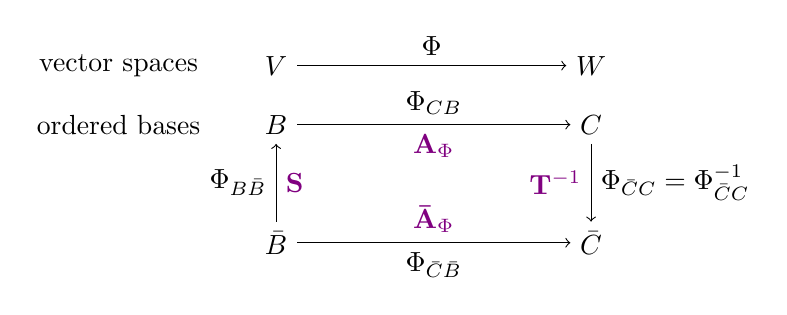
\begin{tikzpicture}[x=2cm, y=0.75cm]
                        \node[] (v) at (0, 0) {$V$};
                        \node[] (w) at (2, 0) {$W$};
                        \node[] (b) at (0, -1) {$B$};
                        \node[] (c) at (2, -1) {$C$};
                        \node[] (bb) at (0, -3) {$\bar{B}$};
                        \node[] (cb) at (2, -3) {$\bar{C}$};
                        \node[] () at (-1, 0) {vector spaces};
                        \node[] () at (-1, -1) {ordered bases};
                        \draw
                        (v) edge[->] node[above] {$\Phi$} (w)
                        (b) edge[->] node[above] {$\Phi_{CB}$} node[below] {\textcolor{violet}{$\mat{A}_\Phi$}} (c)
                        (bb) edge[->] node[below] {$\Phi_{\bar{C}\bar{B}}$} node[above] {\textcolor{violet}{$\mat{\bar{A}}_\Phi$}} (cb)
                        (bb) edge[->] node[left] {$\Phi_{B\bar{B}}$} node[right] {\textcolor{violet}{$\mat{S}$}} (b)
                        (c) edge[->] node[right] {$\Phi_{\bar{C}C} = \Phi_{\bar{C}C}^{-1}$} node[left] {\textcolor{violet}{$\mat{T}^{-1}$}} (cb);
                    \end{tikzpicture}
                \end{center}
                We say that two matrices, $\mat{A}, \mat{\bar{A}} \in \mathbb{R}^{m \times n}$ are equivalent if there exists regular matrices $\mat{S} \in \mathbb{R}^{n \times n}$, and $\mat{T} \in \mathbb{R}^{m \times m}$, such that $\mat{\bar{A}} = \mat{T}^{-1}\mat{A}\mat{S}$. We say they are similar if $\mat{A}, \mat{\bar{A}} \in \mathbb{R}^{n \times n}$, has a corresponding regular matrix $\mat{S} \in \mathbb{R}^{n \times n}$, such that $\mat{\bar{A}} = \mat{S}^{-1}\mat{A}\mat{S}$. Therefore, it follows that similarity is a stronger property than equivlance, since all similar matrices are equivalent, but not vice versa.
                \medskip

                With $\mathbb{R}$-vector spaces $V, W, X$, mappings $\Phi : V \to W$, $\Psi : W \to X$; we define the composed mapping $\Psi \circ \Phi : V \to X$, to have the transformation matrix $\mat{A}_{\Psi \circ \Phi} = \mat{A}_\Psi \mat{A}_\Phi$
                % todo: worked example on page 76/80 of notes
            \subsubsection*{Determinants}
                Determinants are only defined for square matrices $\mat{A} \in \mathbb{R}^{n \times n}$, and will be denoted as $\text{det}(\mat{A})$, or $|\mat{A}|$. There are also some properties about determinants of smaller matrices, but I'm skipping that.
                \begin{center}
                    $\mat{A} =\begin{bmatrix}
                        a_{1,1} & a_{1,2} & \cdots & a_{1, n} \\
                        0 & a_{2,2} & \cdots & a_{2, n} \\
                        \vdots & \ddots & \ddots & \vdots \\
                        0 & \cdots & 0 & a_{n, n}
                    \end{bmatrix}$ is an upper triangular matrix, therefore $\text{det}(\mat{A}) = \prod\limits_{i=1}^{n}{a_{i, i}}$
                \end{center}
                We can also apply the following properties of determinants, without proof;
                \begin{itemize}
                    \itemsep0em
                    \item $\text{det}(\mat{A}\mat{B}) = \text{det}(\mat{A}) \cdot \text{det}(\mat{B})$
                    \item $\text{det}(\mat{A}) = 0 \Leftrightarrow \mat{A}$ is singular (hence $\text{det}(\mat{A}) \neq 0 \Leftrightarrow $ if it is regular)
                    \item $\text{det}(\mat{A}) = \text{det}(\mat{A}^\top)$
                    \item if $\mat{A}$ is regular; $\text{det}(\mat{A}^{-1}) = \text{det}(\mat{A})^{-1}$
                    \item similar matrices have the same determinant; therefore all $\mat{A}_\Phi$ of $\Phi : V \to V$ have the same determinant
                \end{itemize}
                In order to get the determinant of a matrix by using the triangular form, we can use Gaussian elimination, with the following row operation rules;
                \begin{itemize}
                    \itemsep0em
                    \item adding a multiple of a column/row to another doesn't change $\text{det}(\mat{A})$
                    \item multiplying a column/row by $\lambda \in \mathbb{R}$ scales $\text{det}(\mat{A})$ by $\lambda$, hence $\text{det}(\lambda\mat{A}) = \lambda^n\text{det}(\mat{A})$
                    \item swapping two columns/rows changes the sign of $\text{det}(\mat{A})$
                \end{itemize}
                For example, consider the following sequence of row operations;
                \begin{tabularx}{\textwidth}{llllll}
                    $\begin{vmatrix}
                        2 & 0 & 1 & 2 & 0 \\
                        2 & -1 & 0 & 1 & 1 \\
                        0 & 1 & 2 & 1 & 2 \\
                        -2 & 0 & 2 & -1 & 2 \\
                        2 & 0 & 0 & 1 & 1
                    \end{vmatrix} \begin{matrix}
                        {} \\ -R_1 \\ {} \\ +R_1 \\ -R_1
                    \end{matrix}$ & $\leadsto$ & $\begin{vmatrix}
                        2 & 0 & 1 & 2 & 0 \\
                        0 & -1 & -1 & -1 & 1 \\
                        0 & 1 & 2 & 1 & 2 \\
                        0 & 0 & 3 & 1 & 2 \\
                        0 & 0 & -1 & -1 & 1
                    \end{vmatrix} \begin{matrix}
                        {} \\ {} \\ +R_1 \\ {} \\ {}
                    \end{matrix}$ & $\leadsto$ & $\begin{vmatrix}
                        2 & 0 & 1 & 2 & 0 \\
                        0 & -1 & -1 & -1 & 1 \\
                        0 & 0 & 1 & 0 & 3 \\
                        0 & 0 & 3 & 1 & 2 \\
                        0 & 0 & -1 & -1 & 1
                    \end{vmatrix} \begin{matrix}
                        {} \\ {} \\ {} \\ -3R_3 \\ +R_3
                    \end{matrix}$ & $\leadsto$ \medskip \\

                    $\begin{vmatrix}
                        2 & 0 & 1 & 2 & 0 \\
                        0 & -1 & -1 & -1 & 1 \\
                        0 & 0 & 1 & 0 & 3 \\
                        0 & 0 & 0 & 1 & -7 \\
                        0 & 0 & 0 & -1 & 4
                    \end{vmatrix} \begin{matrix}
                        {} \\ {} \\ {} \\ {} \\ +R_4
                    \end{matrix}$ & $\leadsto$ & $\begin{vmatrix}
                        2 & 0 & 1 & 2 & 0 \\
                        0 & -1 & -1 & -1 & 1 \\
                        0 & 0 & 1 & 0 & 3 \\
                        0 & 0 & 0 & 1 & -7 \\
                        0 & 0 & 0 & 0 & -3
                    \end{vmatrix}$ & $=$ & $2 \cdot -1 \cdot 1 \cdot 1 \cdot -3 = 6$\\
                \end{tabularx}
                Another method for calculating the determinant of a matrix is via \textbf{Laplace Expansion}. We define a matrix $\mat{A} \in \mathbb{R}^{n \times n} = (a_{i,j})$, and another matrix $\mat{A}_{i, j} \in \mathbb{R}^{(n - 1) \times (n - 1)}$ as $\mat{A}$ without its $i^\text{th}$ row, nor its $j^\text{th}$ column.
                \begin{itemize}
                    \itemsep 0em
                    \item $\text{det}(\mat{A}) = \summation{k = 1}{n}{(-1)^{k + j}a_{i, k}\text{det}(\mat{A}_{i, k})}$ \hfill expansion along row $i$
                    \item $\text{det}(\mat{A}) = \summation{k = 1}{n}{(-1)^{k + j}a_{k, j}\text{det}(\mat{A}_{k, j})}$ \hfill expansion along column $j$
                \end{itemize}
                The checkerboard pattern formed by the signs are as follows, for $\mat{A} \in \mathbb{R}^{n \times n}$;
                \begin{center}
                    $n$ is odd; $\begin{bmatrix}
                        + & - & \cdots & + \\
                        - & + & \cdots & - \\
                        \vdots & \vdots & \ddots & \vdots \\
                        + & - & \cdots & +
                    \end{bmatrix}$, or when $n$ is even; $\begin{bmatrix}
                        + & - & \cdots & - \\
                        - & + & \cdots & + \\
                        \vdots & \vdots & \ddots & \vdots \\
                        - & + & \cdots & +
                    \end{bmatrix}$
                \end{center}
                It's better to expand along rows/columns with as many 0s as possible, as that would reduce the amount of work that needs to be done.
            \subsubsection*{Eigenvalues, and Eigenvectors}
                We define $\lambda$ as an eigenvalue for an endomorphism $\Phi : V \to V$, $\Leftrightarrow \exists \vec{v} \in V \vec{0} [\vec{v} \neq \vec{0} \land \Phi(\vec{v}) = \lambda \vec{v}]$. The set of all eigenvectors corresponding to some $\lambda$ in $\mat{A}_\Phi$ is defined as the \textbf{eigenspace} of $\mat{A}_\Phi$, with respect to $\lambda$, and is written as $E_\lambda$. The set of all eigenvalues of $\mat{A}_\Phi$ is called the \textbf{spectrum} of $\mat{A}_\Phi$.
                \medskip

                We can also say that $\lambda$ is an eigenvalue of $\mat{A}$, when $\text{rk}(\mat{A} - \lambda \mat{I}_n) < n$, hence $\text{det}(\mat{A} - \lambda \mat{I}_n) = 0$.
                \medskip

                From the latter definition, we can define the characteristic polynomial $p(\lambda) \triangleq \text{det}(\mat{A} - \lambda \mat{I}_n)$. By setting $p(\lambda) = 0$, the roots of our equations are the eigenvalues of $\mat{A}$.
                \medskip

                To determine the eigenspace of $\mat{A}_\Phi$, with eigenvalue $\lambda$, we take $\text{ker}(\mat{A}_\Phi - \lambda \mat{I}_n)$. Since we defined an eigenvalue to satisfy $\mat{A}_\Phi \vec{x} = \lambda \vec{x} \Leftrightarrow (\mat{A}_\Phi - \lambda \mat{I}_n)\vec{x} = \vec{0}$, so we're simply solving a homogeneous system of equations.
                \medskip

                We can say that two similar matrices $\mat{A}, \mat{\bar{A}} \in \mathbb{R}^{n \times n}$, have the same characteristic polynomial;
                \begin{reasoning}
                    \proofmath{\text{det}(\mat{\bar{A}} - \lambda \mat{I}_n)}{\text{det}(\mat{S}^{-1}\mat{A}\mat{S} - \lambda \mat{I}_n)}{by definition of similar matrices}
                    \proofmath{}{\text{det}(\mat{S}^{-1}\mat{A}\mat{S} - \lambda \mat{S}^{-1}\mat{I}_n\mat{S})}{$\mat{S}^{-1}\mat{S} = \mat{I}_n$}
                    \proofmath{}{\text{det}(\mat{S}^{-1}(\mat{A} -\lambda \mat{I}_n)\mat{S})}{distributivity of matrix multiplication}
                    \proofmath{}{\text{det}(\mat{S}^{-1})\cdot\text{det}(\mat{A} -\lambda \mat{I}_n)\cdot\text{det}(\mat{S})}{property of determinants}
                    \proofmath{}{\text{det}(\mat{S})^{-1}\cdot\text{det}(\mat{A} -\lambda \mat{I}_n)\cdot\text{det}(\mat{S})}{property of determinants}
                    \proofmath{}{\text{det}(\mat{A} -\lambda \mat{I}_n)}{}
                \end{reasoning}
                There are some worked examples in the notes, but this is something that \textbf{needs} to be practiced. The concept itself isn't too difficult, but being able to apply it quickly needs some practice.

\end{document}
